% Estas slides tienen que abrirse con el programa pdfpc que soporta videos embebidos. Para los videos se requiere ubuntu-restricted-extras. El comando es: pdfpc -g slides.pdf

% compress: Encabezado muestra solo la section actual
\documentclass[compress]{beamer}
\mode<presentation>

\usetheme{Copenhagen}
\useoutertheme{taihu}
\useinnertheme{rectangles}

% Itemize configuration
\setbeamertemplate{itemize item}[rectangle]
\setbeamertemplate{itemize subitem}[circle]
\setbeamertemplate{itemize subsubitem}[triangle]

\setbeamertemplate{navigation symbols}{} % Remover símbolos de navegación
\usefonttheme[onlymath]{serif} % Símbolos matemáticos en Serif

\setbeamertemplate{blocks}[rounded] % Block corners rounded
\setbeamercolor{block body}{bg=blue!12,fg=black} % Color of blocks

\usepackage{pdfpc-commands} % pdfpc movie commands
\usepackage[utf8]{inputenc}
\usepackage[spanish]{babel}
\usepackage[binary-units=true]{siunitx} % Para manejar las unidades
\usepackage{multirow}
\usepackage{multimedia}
\usepackage{graphicx}
\usepackage{xcolor}
\usepackage{booktabs} % \toprule

% Elimina la palabra 'Figura' del caption
\usepackage[caption=false]{subfig}
\setbeamertemplate{caption}{\raggedright\insertcaption\par}
\captionsetup[subfigure]{labelformat=empty} % Remover índice del caption de la subfigura

\usepackage{import} % Para el comando import (se usa para pdf_tex)

% Para notas personales en el pdfpc
\usepackage{pdfpcnotes}

\AtBeginSection[]
{
   \begin{frame}
       \frametitle{Índice}
       \tableofcontents[currentsection]
   \end{frame}
}

\setbeamercovered{transparent}

\usepackage{amsmath}
\usepackage{amssymb}
\usepackage{amsopn}

% math
\renewcommand{\vec}[1]{\boldsymbol{\mathbf{#1}}}
\newcommand{\norm}[1]{\left\lVert#1\right\rVert}

% Declare arg max and arg min functionss
\DeclareMathOperator*{\argmax}{arg\,max}
\DeclareMathOperator*{\argmin}{arg\,min}

% Homogeneous decoration function
\newcommand{\homo}[1]{\dot{#1}}

% Declare projection as math function
\DeclareMathOperator{\proj}{proj}
\DeclareMathOperator{\disp}{disp}
\newcommand{\worldCoordSystem}{\mathrm{w}}
\newcommand{\cameraCoordSystem}{\mathrm{c}}
\newcommand{\point}{\vec{x}}
\newcommand{\worldPoint}{\point^{\mathrm{w}}}
\newcommand{\homoWorldPoint}{\homo{\point}^{\mathrm{w}}}
\newcommand{\cameraPoint}{\point^{\mathrm{c}}}
\newcommand{\hatCameraPoint}{\hat{\point}^{\mathrm{c}}}
\newcommand{\homoCameraPoint}{\homo{\point}^{\mathrm{c}}}
\newcommand{\measurement}{\vec{z}}
\newcommand{\prediction}{\hat{\vec{z}}}
\newcommand{\imagePoint}{\vec{u}}
\newcommand{\seMatrix}{\vec{E}}
\newcommand{\rotation}{\vec{R}}
\newcommand{\translation}{\vec{t}}
\newcommand{\intrinsicMatrix}{\vec{K}}
\newcommand{\principalPoint}{\vec{c}}
\newcommand{\reprojectionError}{u}
\newcommand{\projectionMatrix}{\vec{P}}
\newcommand{\cameraCenter}{\vec{o}}


% Dense Map
\newcommand{\current}{\mathrm{current}}
\newcommand{\previous}{\mathrm{previous}}
\newcommand{\fusion}{\mathrm{fusion}}
\newcommand{\inverseDepth}{\rho}
\newcommand{\plane}{\boldsymbol{\pi}}
\newcommand{\reference}{ref}


% scaled operators and letters to fancy view
\newcommand{\sminus}{\scalebox{0.5}[1.0]{$-$}}
\newcommand{\splus}{\scalebox{0.6}[0.6]{$+$}}
\newcommand{\curr}{c}
\newcommand{\sind}[1]{\scalebox{0.6}[0.6]{$#1$}}
\newcommand{\ind}[1]{\scalebox{0.7}[0.7]{$#1$}}

\newcommand{\keyframe}{\vec{K}}
\newcommand{\pointCloud}{\mathcal P}
\newcommand{\groundTruth}[1]{{#1}^{*}}

\newcommand{\update}[1]{\hat{#1}}

\newcommand{\position}{\vec{p}}
\newcommand{\map}{M}

\newcommand{\baseline}{b}
\newcommand{\focalDistance}{f}
\newcommand{\disparityMap}{\mathcal D}
\newcommand{\camera}{c}
\newcommand{\ray}{n}


\setbeamerfont{normal text}{size*={10}{10}}
\AtBeginDocument{\usebeamerfont{normal text}}

\title{Mapeo denso en tiempo real sobre sistemas SLAM basados en visión estéreo}
\author{Ariel D'Alessandro}
\institute{Director: Taihú Pire. Co-Director: Rodrigo Baravalle. \\ \vspace{0.5cm} Tesina de Grado \\ Licenciatura en Ciencias de la Computación \\ FCEIA - UNR}
\titlegraphic{
\includegraphics[width=0.14\textwidth]{images/logo-unr.png}}
\date{\scriptsize{22 de diciembre de 2017}}

\begin{document}

\frame{\titlepage}


% Frame ---------------------------------------------------------------------
\begin{frame}
\frametitle{Índice}
\tableofcontents
\end{frame}


\section{Introducción}


\subsection{Motivación}


% Frame ---------------------------------------------------------------------
\begin{frame}
	\frametitle{Motivación}
	
	Problema de la robótica móvil
	\begin{itemize}
		\item Planeamiento de una trayectoria segura hacia determinados objetivos.
		\item Debe hacerse a medida que el robot se desplaza a través de un entorno potencialmente desconocido.
		\item Para esto resulta necesario contar con:
		\begin{itemize}
			\item Una representación del ambiente que se está transitando (mapa).
			\item La ubicación del robot dentro de este mapa.
			\item El mapa debe ser lo suficientemente detallado (denso) para que el robot pueda realizar un planeamiento seguro, evitando posibles obstáculos.
		\end{itemize}
	\end{itemize}
\end{frame}


\subsection{SLAM}


% Frame ---------------------------------------------------------------------
\begin{frame}
	\frametitle{SLAM: Simultaneous Localization and Mapping}
    \begin{itemize}
        \item ¿Qué es SLAM?
        \begin{itemize}
            \item Localización y Mapeo Simultáneos.
        \end{itemize}
        \item ¿Por qué es importante en la robótica móvil? 
    \end{itemize}

    \begin{itemize}
            \item Tipos de sensores
            \begin{itemize}
                \item Cámaras.
				\item Sonares.
				\item Láser.
				\item GPS.
				\item Sensores RGB-D.
				\item IMU.
				\item Encoders.
            \end{itemize}
    \end{itemize}

\end{frame}


% Frame ---------------------------------------------------------------------
\begin{frame}
	\frametitle{SLAM - Simultaneous Localisation and Mapping}

	\begin{itemize}
        \item Sensores permiten detectar marcas naturales (\textbf{landmarks})
        \begin{itemize}
            \item El robot determina su posición y orientación en base a estas.
            \item Construye incrementalmente un mapa del entorno, ubicando estas marcas en el mismo.
        \end{itemize}
    \end{itemize}

	\vspace{-1em}
	\begin{figure}[!htb]
		\centering
		\subfloat[]{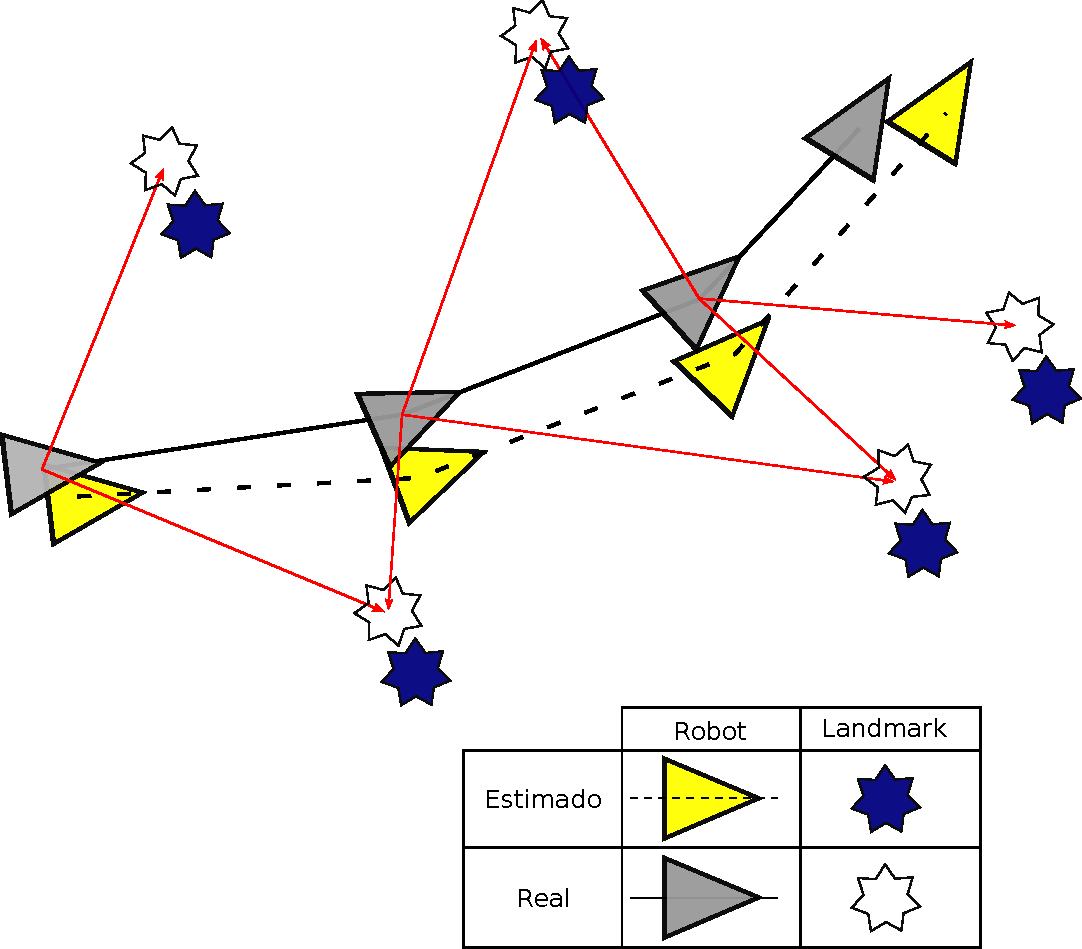
\includegraphics[width=0.6\columnwidth]{./introduction/slam-landmarks.pdf}}
		\hfill
	\end{figure}

\end{frame}


\subsection{SLAM Visual}


% Frame ---------------------------------------------------------------------
\begin{frame}
	\frametitle{SLAM Visual}
    \begin{itemize}
        \item SLAM Visual: Cámaras como sensores
        \begin{itemize}
            \item Obtienen gran cantidad de información del ambiente.
            \item Pueden operar tanto en ambientes interiores como exteriores.
            \item Son sensores pasivos.
            \item De bajo costo y portátiles.
        \end{itemize}
    \end{itemize}
    
    \pause{}
    \begin{itemize}
        \item Ventajas al trabajar con cámaras estéreo        
        \begin{itemize}
            \item Permiten recuperar la profundidad de la escena con una única captura.
            \item Permiten conocer la escala real de la escena observada.
        \end{itemize}
    \end{itemize}
\end{frame}


\subsection{Conceptos básicos}


% Frame ---------------------------------------------------------------------
\begin{frame}
	\frametitle{Modelo de cámara pinhole}

	\begin{block}{Definición - Cámara}
		Una cámara es definida matemáticamente como un mapeo entre puntos del mundo 3D y puntos de la imagen (píxeles).
	\end{block}

	\begin{block}{Cámara pinhole}
		El punto de la imagen $\imagePoint=\begin{bmatrix}u & v\end{bmatrix}^{\top}$ es determinado como la intersección entre el \emph{plano de la imagen} y el rayo que une el punto del mundo 3D $\point=\begin{bmatrix}x & y & z\end{bmatrix}^{\top}$ con el \emph{centro focal} $\cameraCenter$ de la cámara.
	\end{block}

	\vspace{-0.5em}
	\begin{figure}[!htb]
		\centering
		\subfloat[]{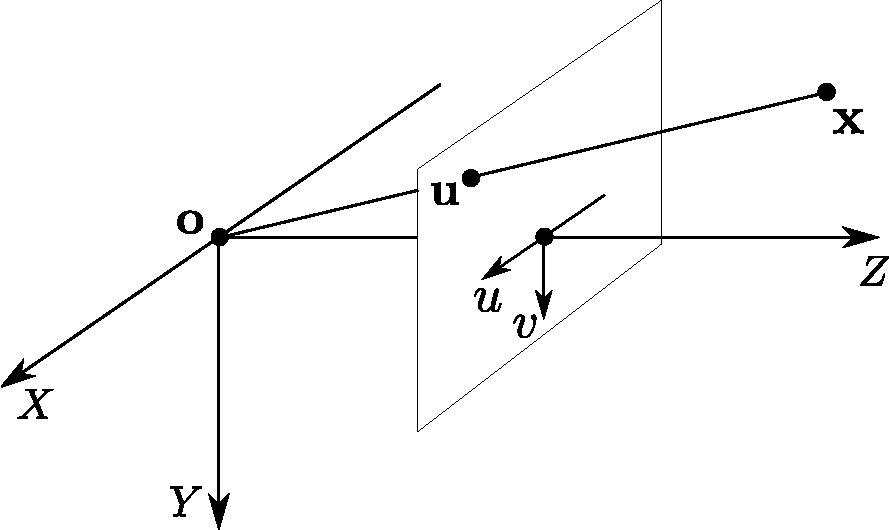
\includegraphics[width=0.5\columnwidth]{./cameras/pinhole_camera_model.pdf}}%
		\hfill
	\end{figure}

\end{frame}


% Frame ---------------------------------------------------------------------
\begin{frame}
	\frametitle{Geometría estéreo}

    \begin{align*}
        \point&=\begin{bmatrix}x & y & z\end{bmatrix}^{\top}
    \end{align*}

	\begin{equation}
		\begin{aligned}x=\frac{(u_{l}-c_{u})z}{f}\;\qquad
		y=\frac{(v_{l}-c_{v})z}{f}\;\qquad
		z=\frac{bf}{u_{l}-u_{r}}\;
		\end{aligned}
	\end{equation}

	\begin{figure}[!htb]
		\centering
		\subfloat[]{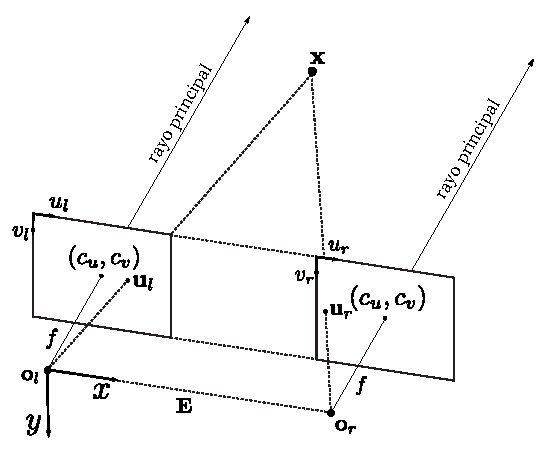
\includegraphics[width=0.5\columnwidth]{./cameras/stereo_rectification.pdf}}%
		\hfill
		\centering
		\subfloat[]{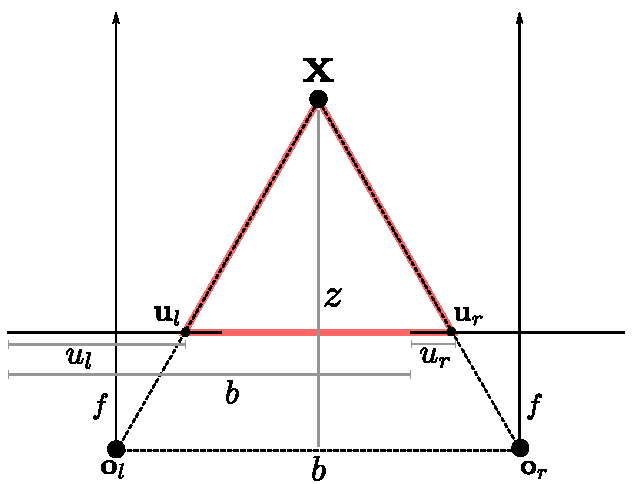
\includegraphics[width=0.5\columnwidth]{./cameras/stereo_triangulation.pdf}}%
		\hfill
	\end{figure}

\end{frame}


% Frame ---------------------------------------------------------------------
\begin{frame}
	\frametitle{Geometría estéreo}

	\begin{block}{Definición - Disparidad}
		Distancia existente entre las proyecciones de las diferentes cámaras.
	\begin{equation}
		d=u_{l}-u_{r}=\frac{bf}{z}
	\end{equation}
	\end{block}

	\textbf{Nota}: la profundidad $z$ es inversamente proporcional a la disparidad $d$.

	\vspace{-1em}
	\begin{figure}[!htb]
		\centering
		\subfloat[]{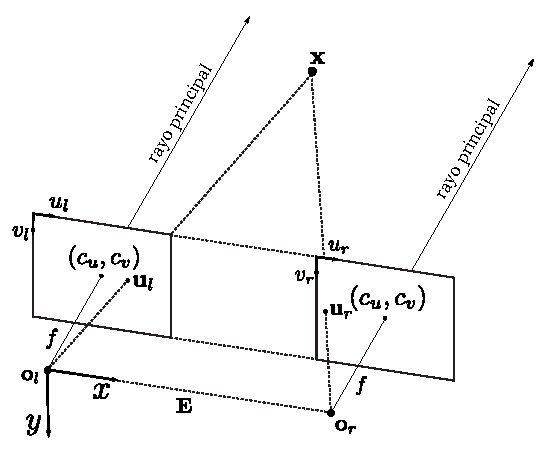
\includegraphics[width=0.5\columnwidth]{./cameras/stereo_rectification.pdf}}%
		\hfill
		\centering
		\subfloat[]{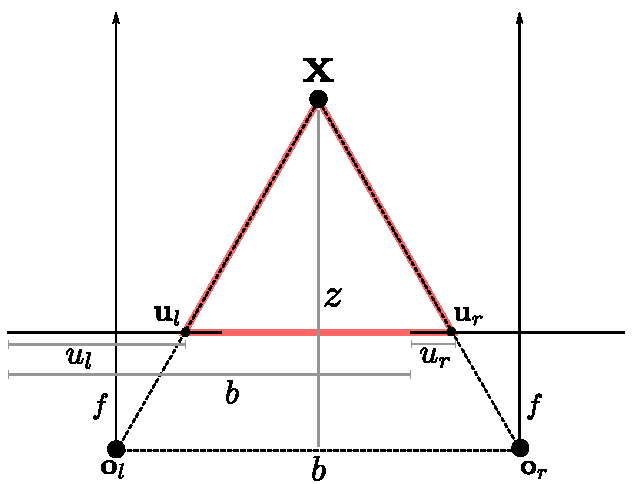
\includegraphics[width=0.5\columnwidth]{./cameras/stereo_triangulation.pdf}}%
		\hfill
	\end{figure}

\end{frame}


\section{S-PTAM Denso}


\subsection{S-PTAM}


% Frame ---------------------------------------------------------------------
\begin{frame}
	\frametitle{S-PTAM}
	\begin{figure}[htb]
		\centering
		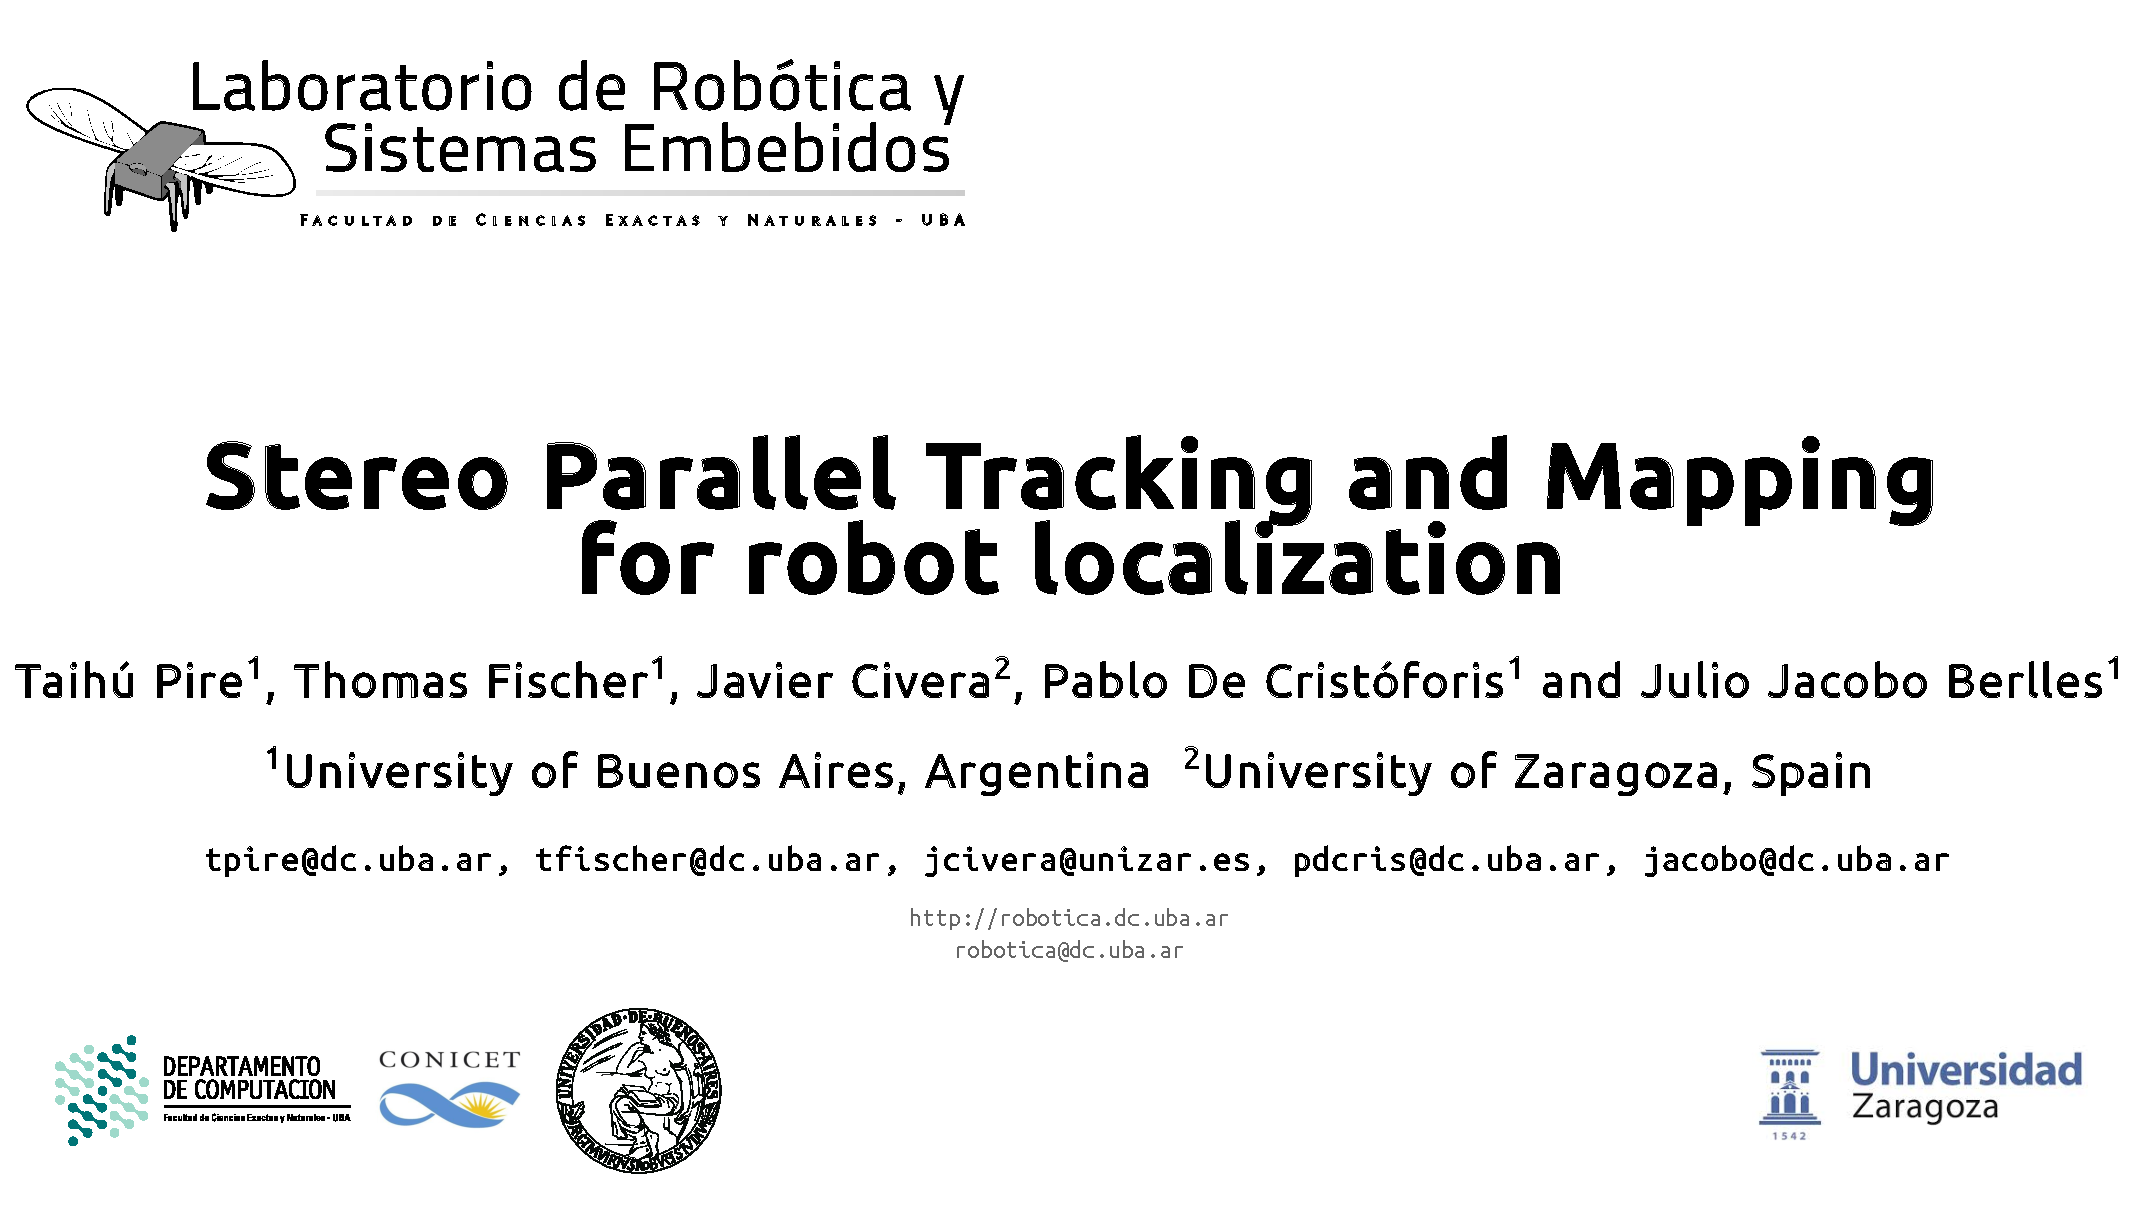
\includegraphics[width=1.0\columnwidth]{method/portada-sptam-kitti-video.pdf}
		\hfill
	\end{figure}

\end{frame}


% Frame ---------------------------------------------------------------------
\begin{frame}
    \frametitle{S-PTAM: Stereo Parallel Tracking and Mapping}
    Características:
    \begin{itemize}
    	\item Sensor: Cámara estéreo
		\item Construye y mantiene un mapa disperso del entorno.
		\item Basado en keyframes.
        \item Sistema SLAM basado en features.
        \item Fuertemente paralelizado: tracking, local mapping y loop closing.
        \item Real-time incluso en trayectorias largas.
        \item Código open-source en ROS (GPLv3) \url{https://github.com/lrse/sptam}
    \end{itemize}
\end{frame}


% Frame ---------------------------------------------------------------------
\begin{frame}
    \frametitle{S-PTAM en acción!}
    TODO: Agregar video de S-PTAM.
\end{frame}


\subsection{Funcionamiento}


% Frame ---------------------------------------------------------------------
\begin{frame}

	\frametitle{S-PTAM Denso}
	\begin{figure}[htb]
		\centering
		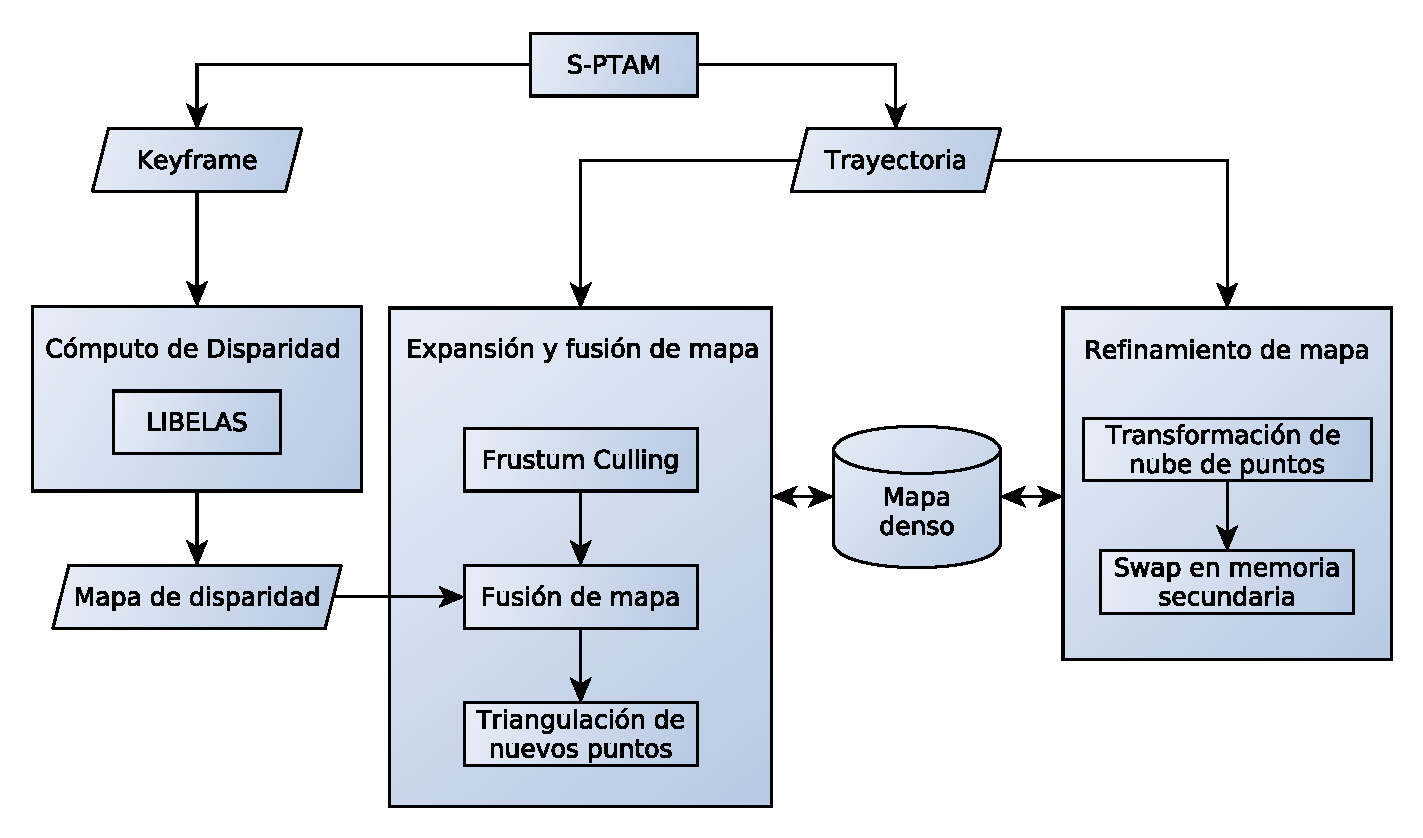
\includegraphics[width=1.0\columnwidth]{method/metodo-diagram.pdf}
		\hfill
	\end{figure}
\end{frame}


% Frame ---------------------------------------------------------------------
\begin{frame}
	\frametitle{Mapa de disparidad}

	\begin{itemize}
		\item Computa mapa de disparidad del \emph{keyframe} actual $\keyframe_{j}$.
	\end{itemize}
	
	\begin{figure}[htb]
		\centering
		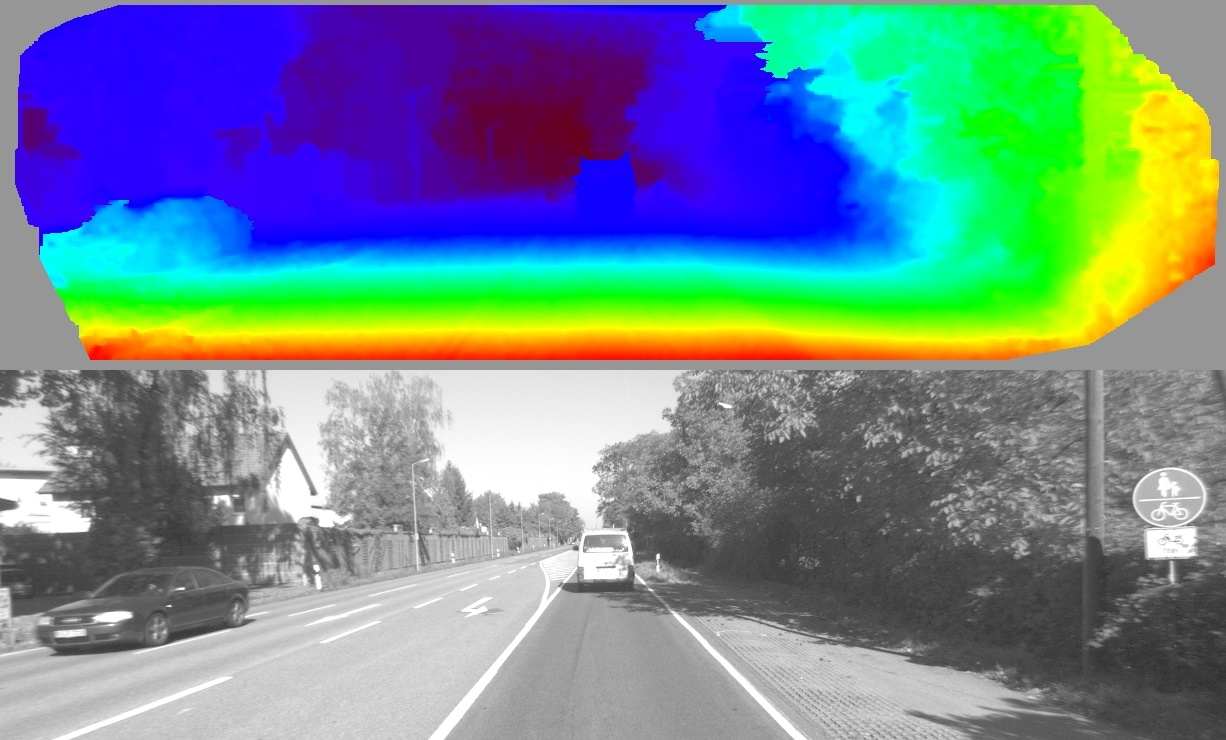
\includegraphics[width=0.4\columnwidth]{method/libelas_merge_kitti04_22.jpg}
		\caption{Mapa de disparidad LIBELAS - Dataset KITTI.}
	\end{figure}

	\begin{figure}[htb]
		\centering
		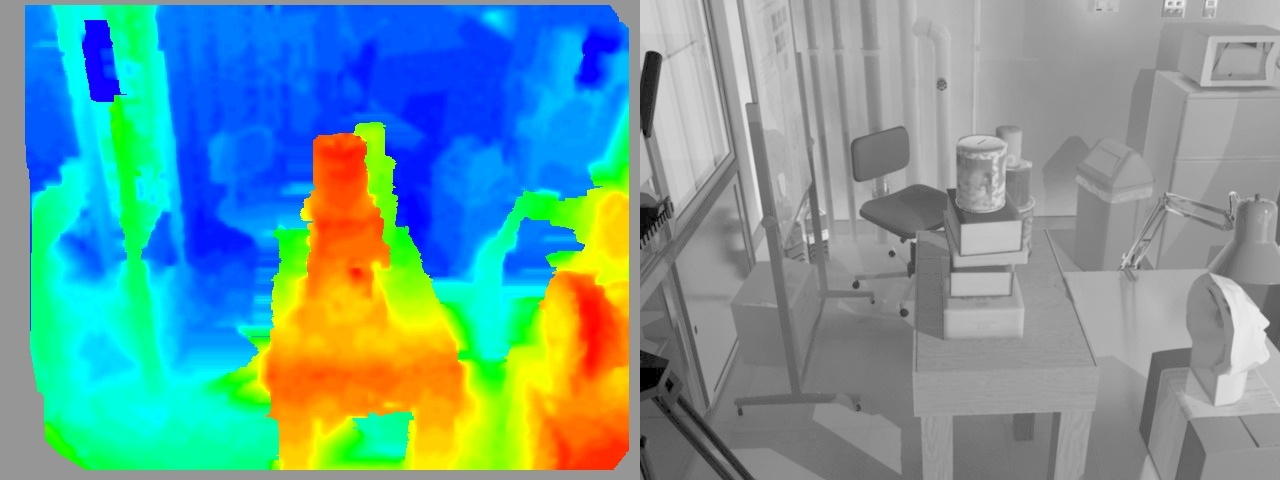
\includegraphics[width=0.4\columnwidth]{method/libelas_merge_tsukuba_222.jpg}
		\caption{Mapa de disparidad LIBELAS - Dataset Tsukuba.}
	\end{figure}

\end{frame}


% Frame ---------------------------------------------------------------------
\begin{frame}
	\frametitle{Expansión y fusión de mapa: Frustrum culling}
	
	\begin{itemize}
		\item Utilizando mapa de disparidad y posición del \emph{keyframe} actual $\keyframe_{j}$.
		\item \emph{Mapa local} a $\keyframe_{j}$: últimas $J$ \emph{nubes de puntos} $\left\{ \pointCloud_{j-J},\hdots,\pointCloud_{j}\right\}$.
		\item Aplicando \emph{Frustum culling} para filtrar puntos no-visibles desde $\keyframe_{j}$.
	\end{itemize}
	
	\begin{figure}[htb]
		\centering
		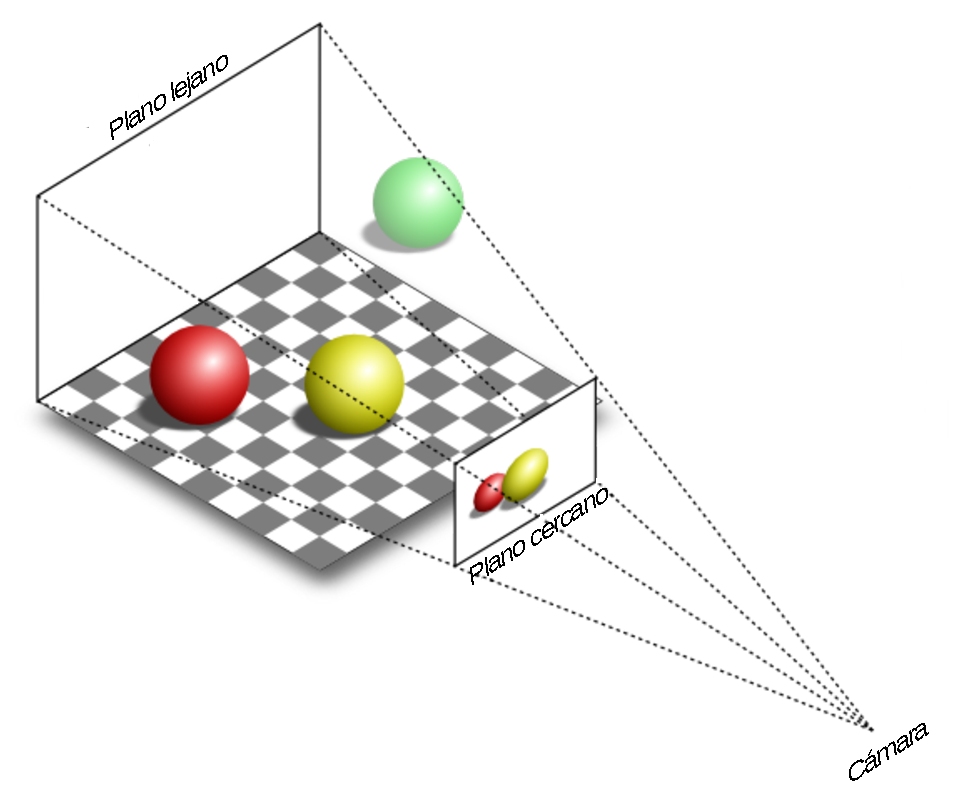
\includegraphics[width=0.6\columnwidth]{method/frustum_culling.pdf}
	\end{figure}

\end{frame}


% Frame ---------------------------------------------------------------------
\begin{frame}
	\frametitle{Expansión y fusión de mapa: Heurística de fusión}
	\begin{figure}[htb]
		\centering
		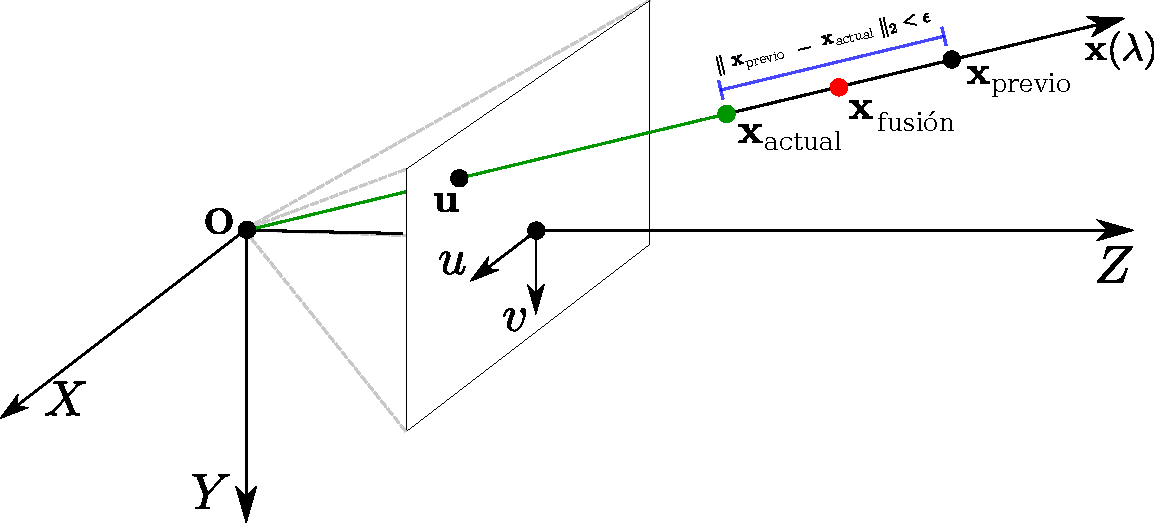
\includegraphics[width=\columnwidth]{method/metodo-fusion-spa.pdf}
	\end{figure}
	\begin{equation*}
		\point_{fusi\acute{o}n}=\frac{1}{\inverseDepth_{fusi\acute{o}n}}\frac{\point_{actual}}{\norm{\point_{actual}}}
		\quad \text{donde} \quad 
		\inverseDepth_{fusi\acute{o}n}=\frac{\inverseDepth_{actual}+\inverseDepth_{previo}}{2}
	\end{equation*}
\end{frame}


% Frame ---------------------------------------------------------------------
\begin{frame}
	\frametitle{Refinamiento de mapa}
	
	Actualización de trayectoria:
	\begin{itemize}
		\item Transforma nubes de puntos cuando la posición del keyframe asociado es actualizada.
		\item Comportamiento esperable en sistemas de SLAM, que refinan la trayectoria a lo largo de la secuencia.
	\end{itemize}

	\vspace{2em}
	\pause{}
	Swap a memoria secundaria:
	\begin{itemize}
		\item Nubes de puntos en RAM hasta que salen del \emph{mapa local}.
		\item Permite secuencias de extensa longitud.
	\end{itemize}

\end{frame}


\subsection{Implementación}


% Frame ---------------------------------------------------------------------
\begin{frame}
	\frametitle{ROS: Robot Operating System}
    \begin{figure}[htb]
        \centering
        
\includegraphics[width=0.55\columnwidth]{method/ros.png}
    \end{figure}
	\vspace{-2em}
    \begin{itemize}
 		\item Conjunto de frameworks para desarrollo de software en robótica.
        \item Abstracción del hardware.
        \item Control de dispositivos de bajo nivel.
        \item Arquitectura:
            \begin{itemize}
	        	\item Cada nodo es una unidad de ejecución.
	        	\item Comunicación entre nodos mediante mensajes.
	        \end{itemize}
        \item Mantenimiento de paquetes.
        \item Utilizado en la comunidad robótica.
    \end{itemize}
\end{frame}


% Frame ---------------------------------------------------------------------
\begin{frame}
	\frametitle{ROS: Robot Operating System}
	
	\begin{figure}[htb]
		\subfloat[] {
			\begin{tabular}[b]{c}
				\centering
				$\vcenter{\hbox{
\includegraphics[width=0.15\columnwidth]{./method/opencv.png}}}$
				\hspace{1em}
				$\vcenter{\hbox{
\includegraphics[width=0.25\columnwidth]{./method/ros.png}}}$
				\hspace{1em}
				$\vcenter{\hbox{
\includegraphics[width=0.25\columnwidth]{./method/pcl.png}}}$
			\end{tabular}
		}
	\end{figure}
	
	\vspace{-2em}
	\begin{itemize}
		\item Implementado como un nodo ROS.
		\item Código fuente disponible públicamente bajo licencia (GPLv3) \url{https://github.com/CIFASIS/dense-sptam}.
		\item Librerías:
		\begin{itemize}
			\item OpenCV: manejo y codificación de imágenes.
			\item Point Cloud Library (PCL): manejo de nubes de puntos.
			\item LIBELAS: cómputo de mapas de disparidad.
		\end{itemize}
		\item Compuesto de 3 hilos de ejecución paralela.
    \end{itemize}
\end{frame}


\section{Evaluación}


\subsection{Datasets}


% Frame ---------------------------------------------------------------------
\begin{frame}
	\frametitle{Dataset KITTI}

	\begin{figure}
		\subfloat[] {
			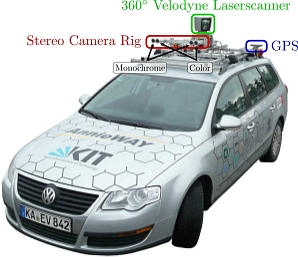
\includegraphics[width=0.3\columnwidth]{./images/kitti_sensors}
		}\hfill{}
		\subfloat[] {
			\begin{tabular}[b]{c}%
				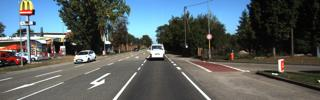
\includegraphics[width=0.3\columnwidth]{./images/kitti01}\thickspace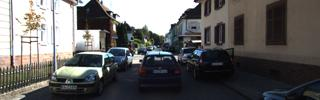
\includegraphics[width=0.3\columnwidth]{./images/kitti02}\\
				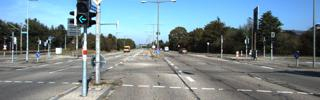
\includegraphics[width=0.3\columnwidth]{./images/kitti03}\thickspace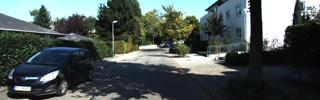
\includegraphics[width=0.3\columnwidth]{./images/kitti04}\\
				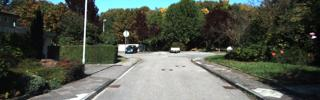
\includegraphics[width=0.3\columnwidth]{./images/kitti05}\thickspace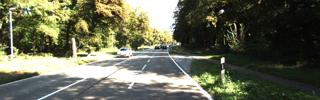
\includegraphics[width=0.3\columnwidth]{./images/kitti06}
			\end{tabular}
		}
	\end{figure}

	\begin{itemize}
        \item Ambientes exteriores (trayectorias de varios kilómetros)
        \item 1344$\times$391@10Hz, baseline: 60cm
    \end{itemize}

\end{frame}


% Frame ---------------------------------------------------------------------
\begin{frame}
	\frametitle{Dataset Tsukuba}

	\begin{figure}
		\subfloat[] {
			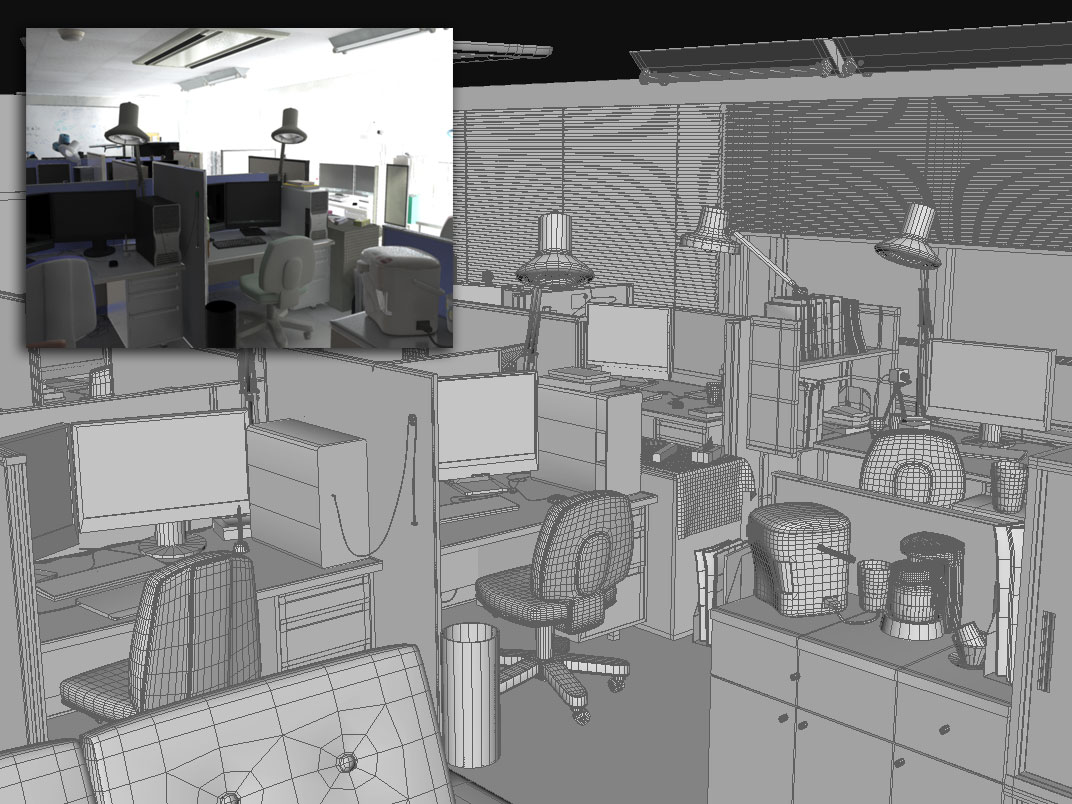
\includegraphics[width=0.41\columnwidth]{./images/tsukuba_dataset}
		}\hspace{0.2cm}
		\subfloat[] {
			\begin{tabular}[b]{c}%
				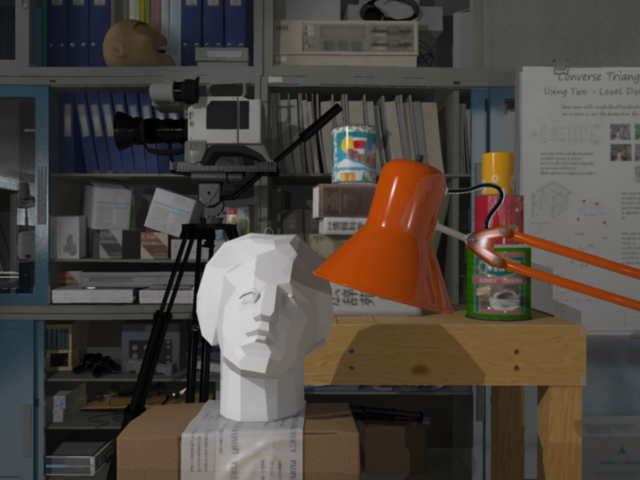
\includegraphics[width=0.2\columnwidth]{./images/tsukuba_sample1}\thickspace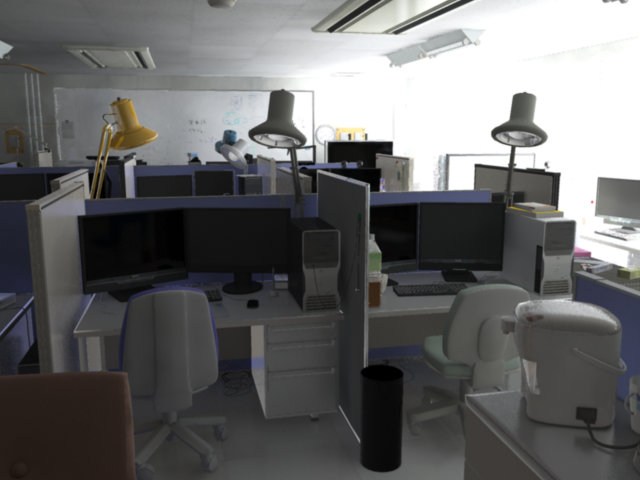
\includegraphics[width=0.2\columnwidth]{./images/tsukuba_sample2}\\
				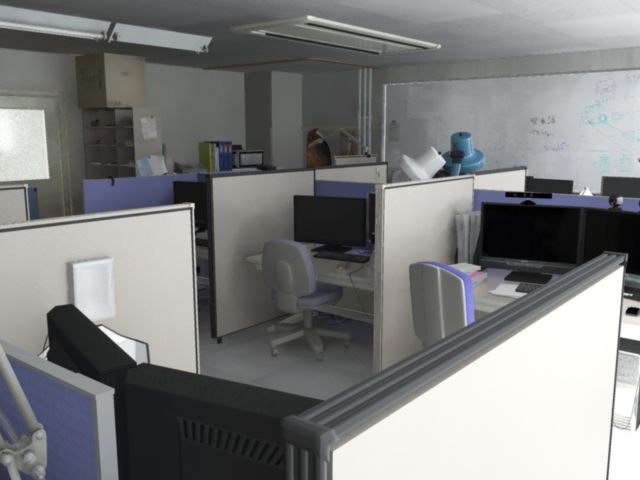
\includegraphics[width=0.2\columnwidth]{./images/tsukuba_sample3}\thickspace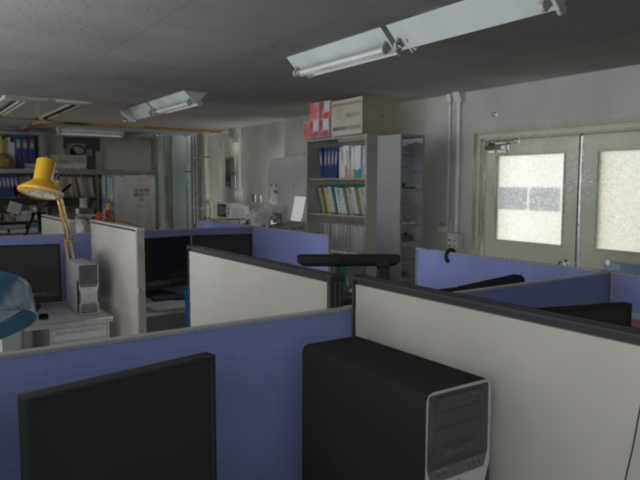
\includegraphics[width=0.2\columnwidth]{./images/tsukuba_sample4}
			\end{tabular}
		}
	\end{figure}
	
	\begin{itemize}
        \item Ambiente interior (sintético)
        \item 640$\times$480@30Hz, baseline: 10cm
    \end{itemize}
    
\end{frame}


% Frame ---------------------------------------------------------------------
\begin{frame}
	\frametitle{Reconstrucción 3D: KITTI}
    TODO: Agregar video de S-PTAM Denso.
\end{frame}


% Frame ---------------------------------------------------------------------
\begin{frame}
	\frametitle{Reconstrucción 3D: Tsukuba}
	\begin{figure}
		\subfloat[] {
			\begin{tabular}[b]{c}
				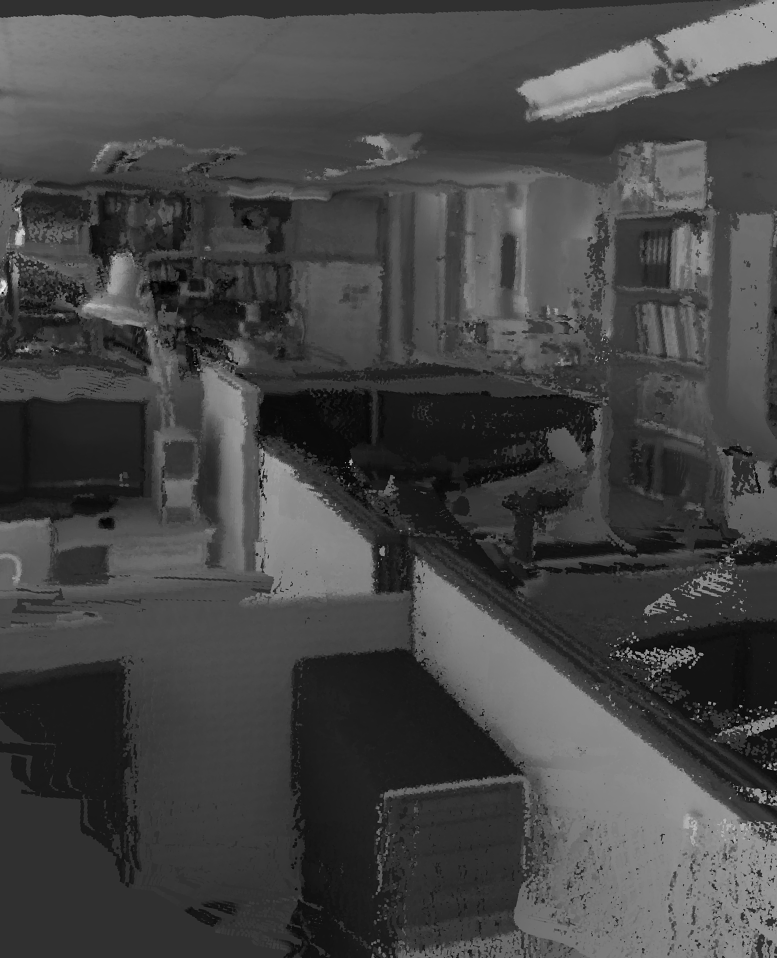
\includegraphics[width=0.3\columnwidth,height=3.0cm]{./images/tsukuba_3d_1}\thickspace
				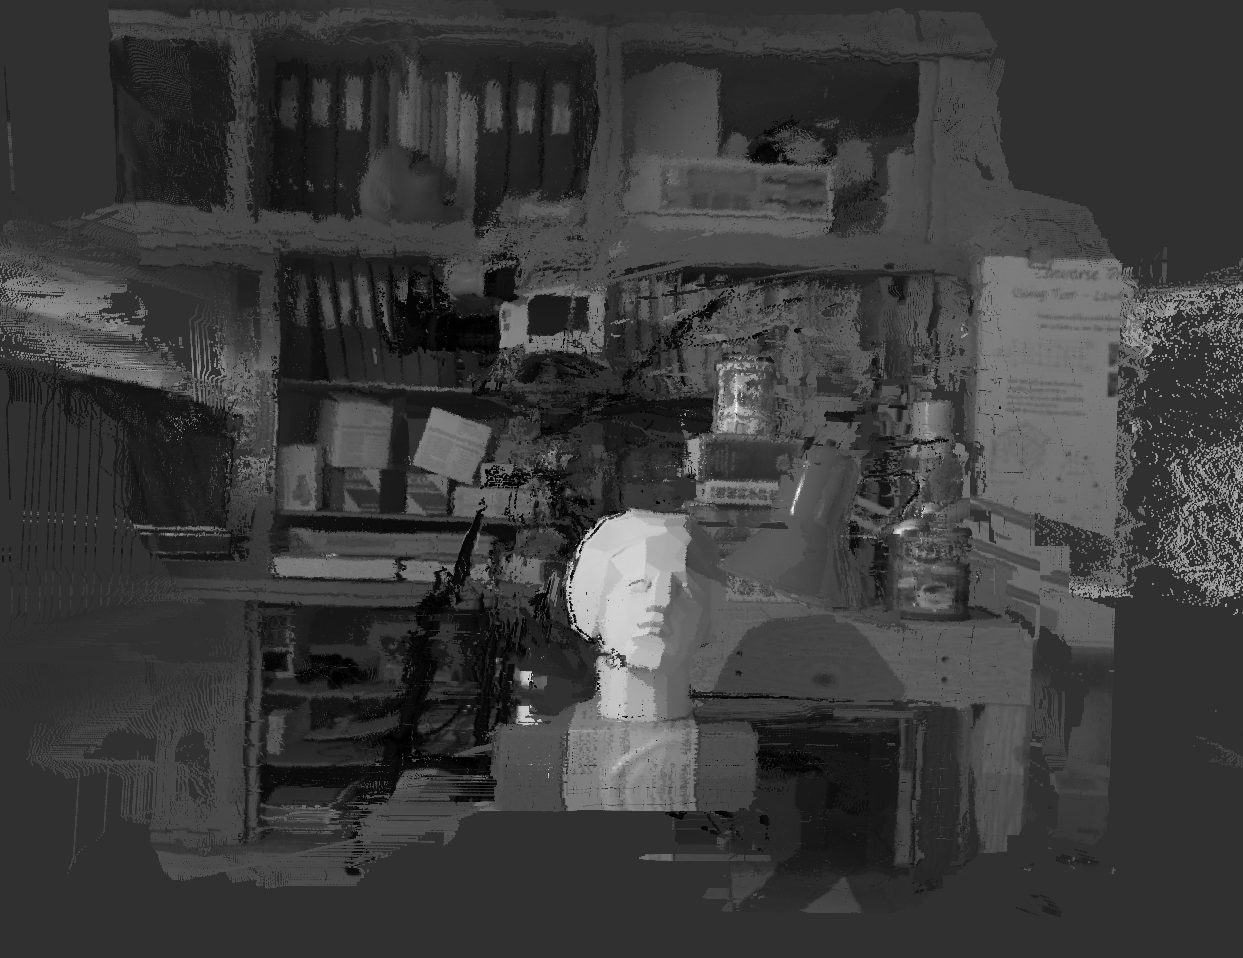
\includegraphics[width=0.3\columnwidth,height=3.0cm]{./images/tsukuba_3d_2}\thickspace
				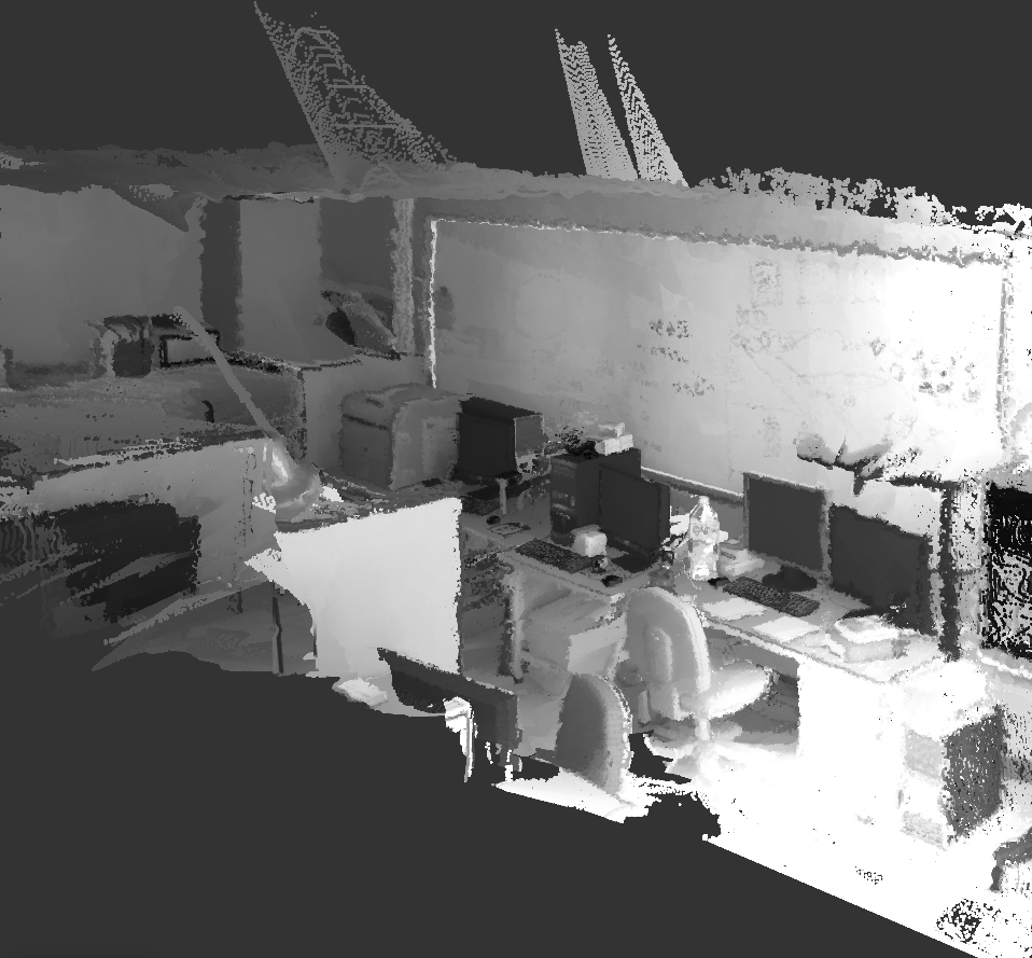
\includegraphics[width=0.3\columnwidth,height=3.0cm]{./images/tsukuba_3d_3}
			\end{tabular}
		}
	\end{figure}
\end{frame}


\subsection{Resultados}


% Frame ---------------------------------------------------------------------
\begin{frame}
	\frametitle{Análisis del error}
	
	\vspace{-1em}
	\pause{}
	Experimentos:
	\begin{itemize}
		\item Comparación de \emph{mapas de profundidad}.
		\item A cada píxel se le asigna el valor de profundidad del punto 3D proyectado.
		\item Generamos un mapa de profundidad para cada keyframe utilizando:
		\begin{itemize}
			\item \emph{Ground truth}.
			\item S-PTAM Denso: proyectando la nubes de puntos global.
			\item LIBELAS: mapa de disparidad.
		\end{itemize}
	\end{itemize}

	\vspace{1em}
	\pause{}	
	KITTI - Ground truth:
	\begin{itemize}
		\item Velodyne: nubes de puntos.
		\item GPS: posición.
	\end{itemize}
	
	\vspace{1em}
	Tsukuba - Ground truth:
	\begin{itemize}
		\item Dataset sintético: provee posición y mapa de profundidad exactos.
	\end{itemize}
	
\end{frame}


% Frame ---------------------------------------------------------------------
\begin{frame}
	\frametitle{KITTI: error de reconstrucción}
	\vspace{-2em}
	\begin{figure}
		\subfloat[Imagen izquierda]{
			\begin{tabular}[b]{c}
				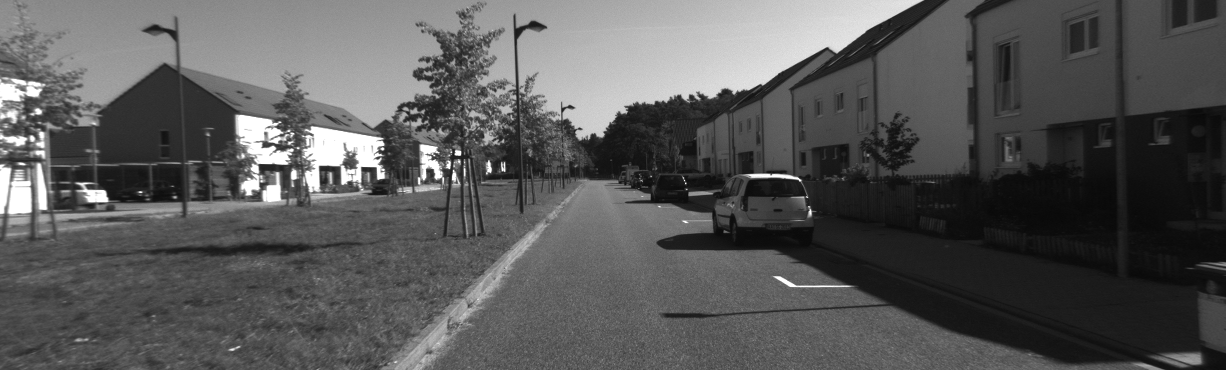
\includegraphics[width=0.45\columnwidth]{./experiments/kitti06_frame612_rgb.png}
			\end{tabular}
		}\thickspace
		\subfloat[Ground-Truth]{
			\begin{tabular}[b]{c}
				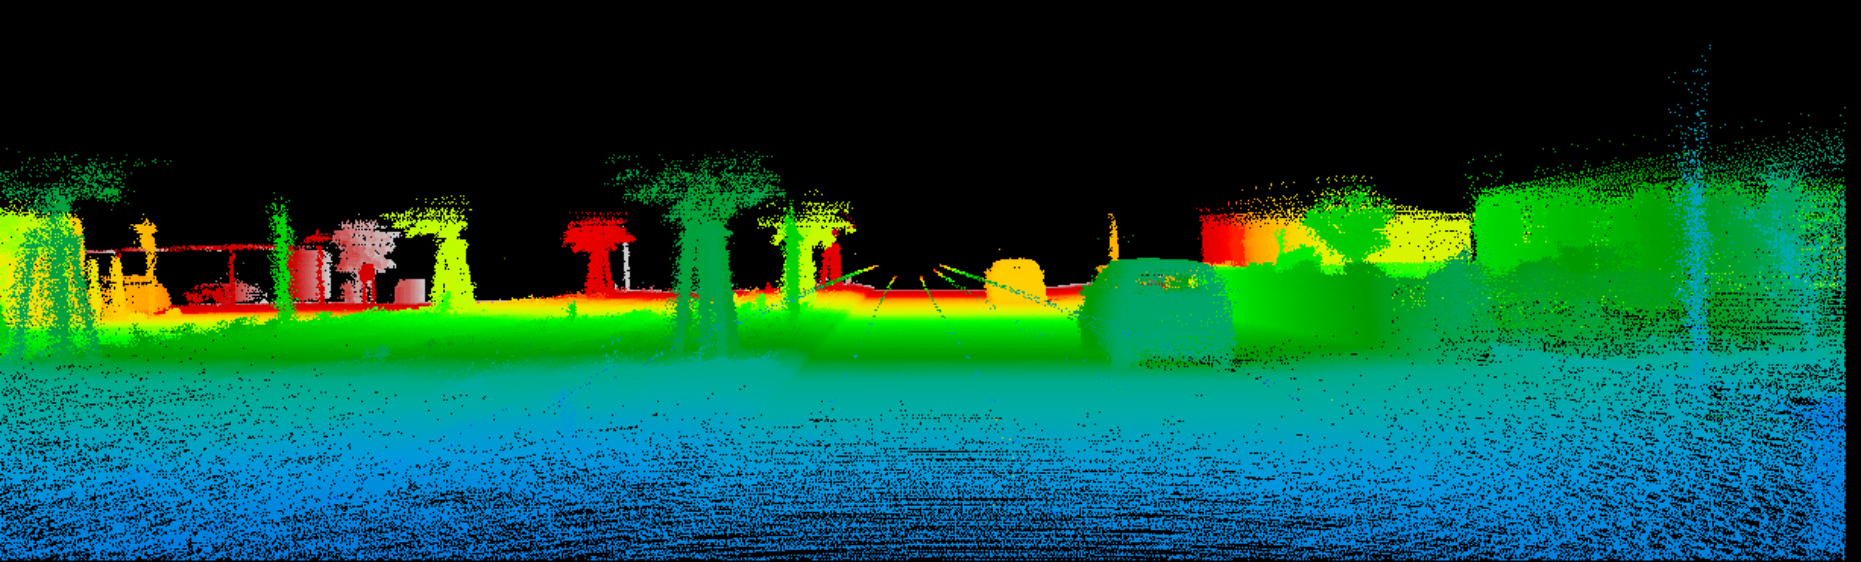
\includegraphics[width=0.45\columnwidth]{./experiments/kitti06_frame612_gt_high50.png}
			\end{tabular}
		}
	\end{figure}
	\vspace{-2em}
	\begin{figure}
		\subfloat[Mapa profundidad LIBELAS]{
			\begin{tabular}[b]{c}
				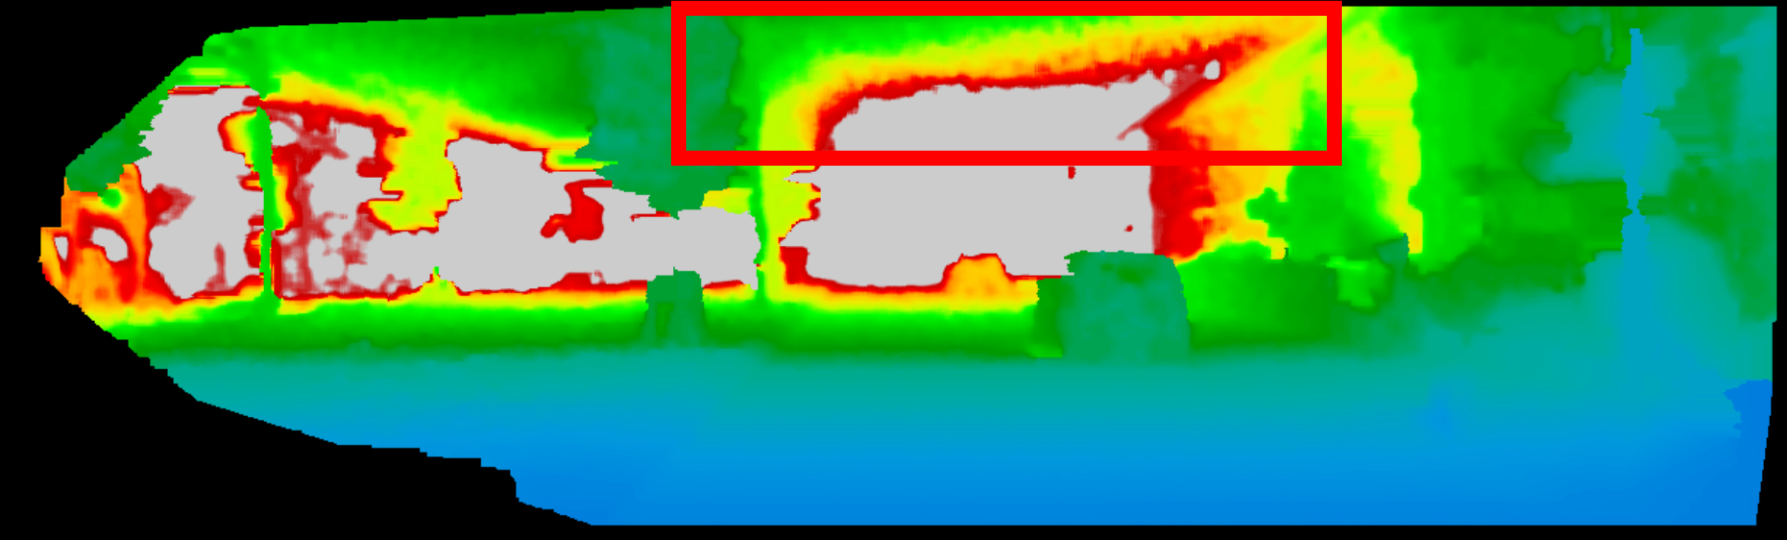
\includegraphics[width=0.45\columnwidth]{./experiments/kitti06_frame612_libelas_depth_high50-m.png}
			\end{tabular}
		}\thickspace
		\subfloat[Error mapa profundidad LIBELAS]{
			\begin{tabular}[b]{c}
				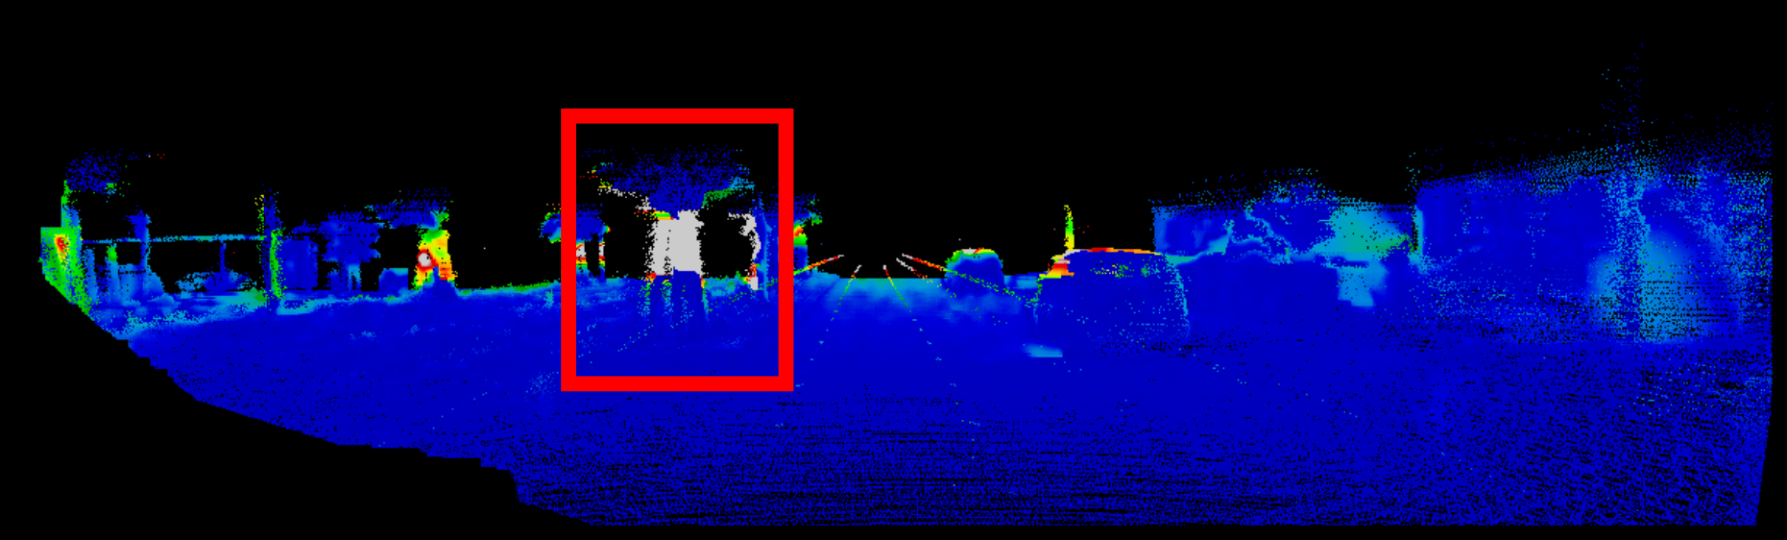
\includegraphics[width=0.45\columnwidth]{./experiments/kitti06_frame612_libelas_error_high50-m.png}
			\end{tabular}
		}
	\end{figure}
	\vspace{-2em}
	\begin{figure}
		\subfloat[Mapa profundidad S-PTAM Denso]{
			\begin{tabular}[b]{c}
				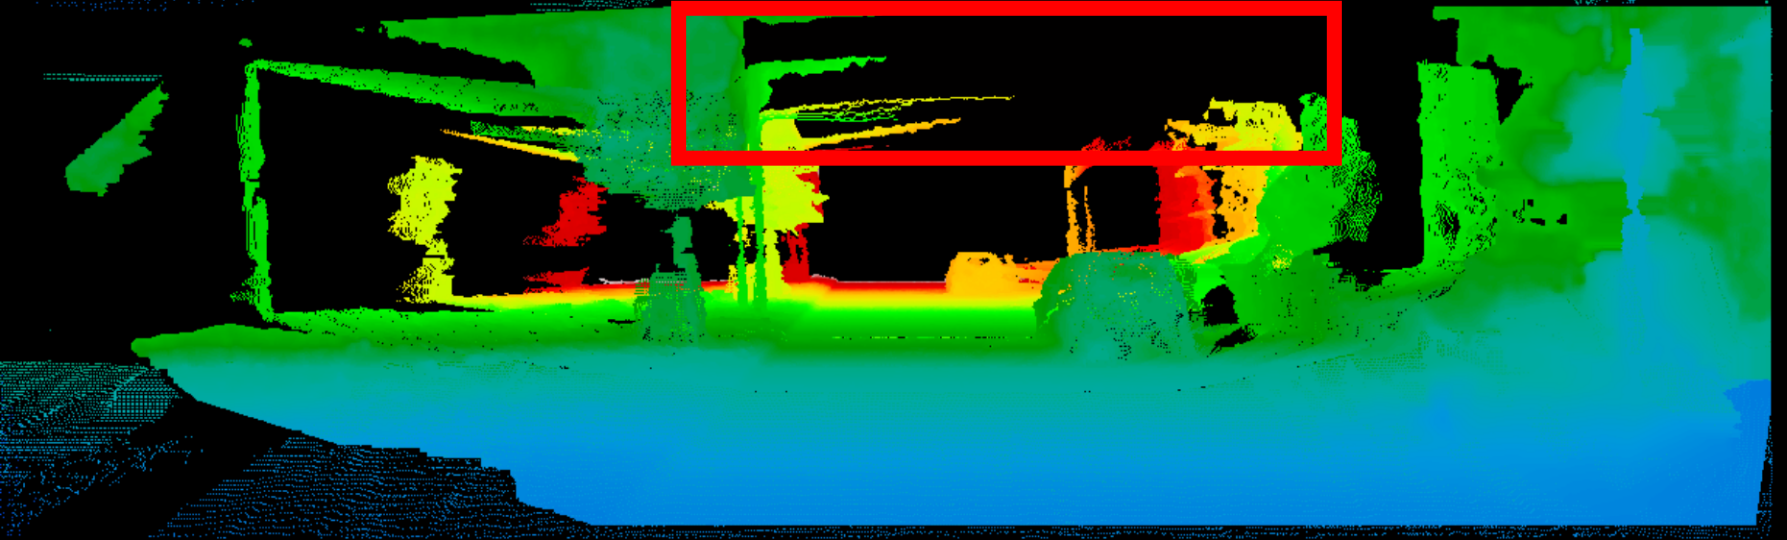
\includegraphics[width=0.45\columnwidth]{./experiments/kitti06_frame612_dense_high50-m.png}
			\end{tabular}
		}\thickspace
		\subfloat[Error mapa profundidad S-PTAM Denso]{
			\begin{tabular}[b]{c}
				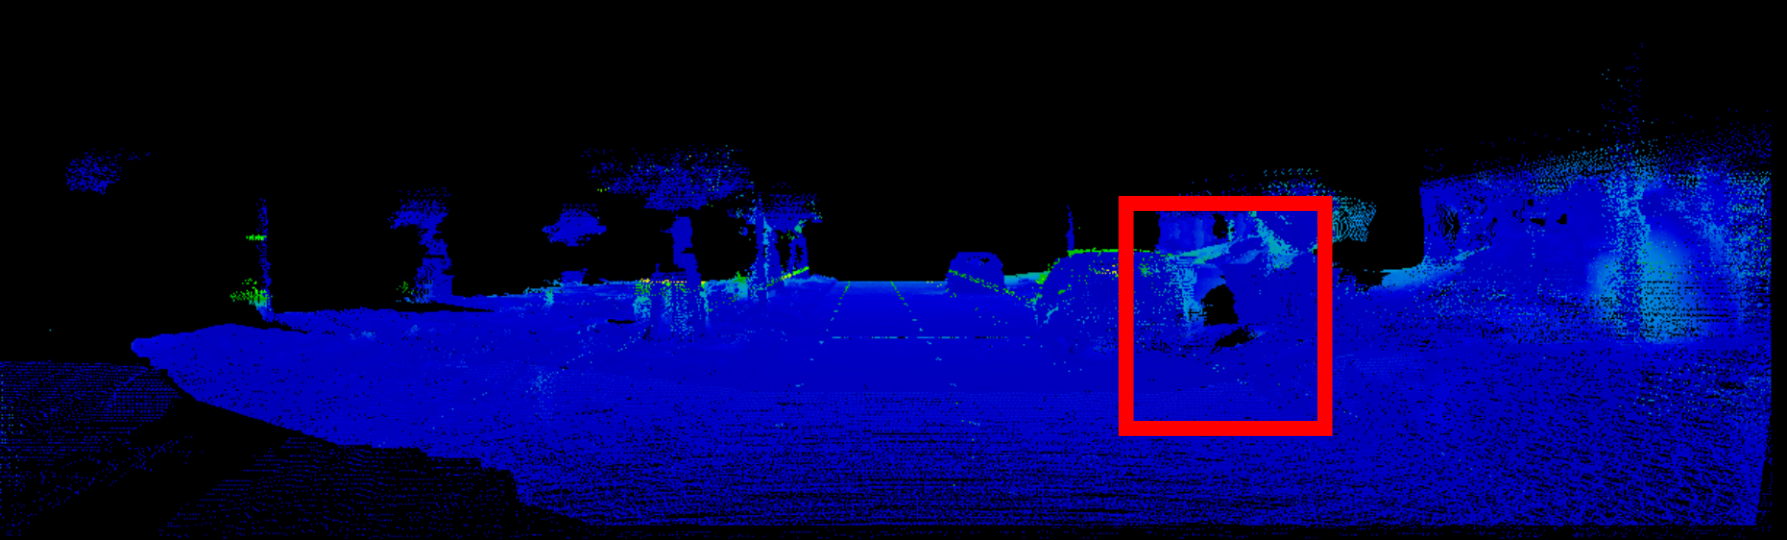
\includegraphics[width=0.45\columnwidth]{./experiments/kitti06_frame612_error_high50-m.png}
			\end{tabular}
		}
	\end{figure}
	\vspace{-2em}
	\begin{figure}
		\subfloat[]{
			\begin{tabular}[b]{c}
				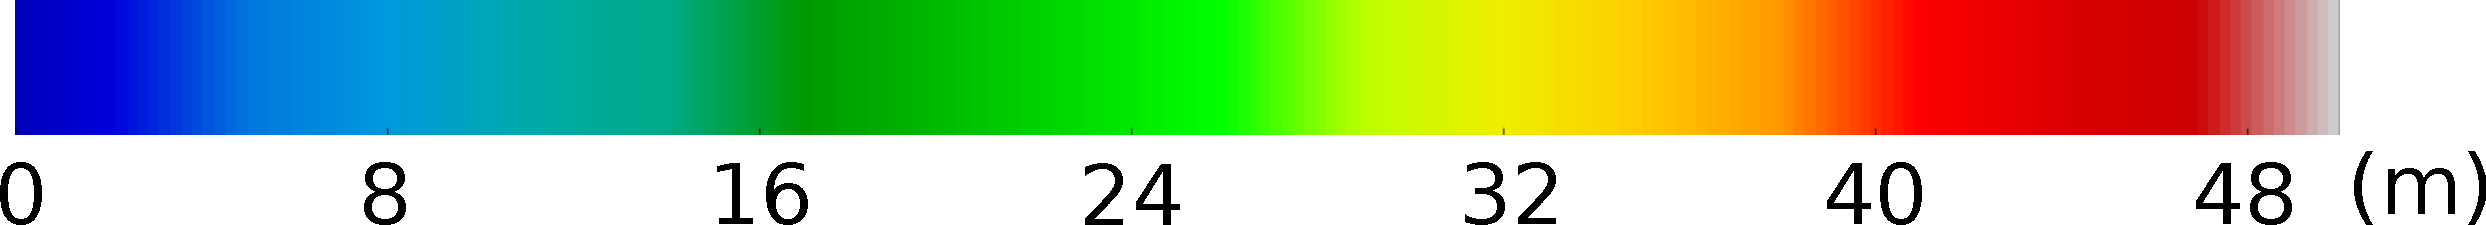
\includegraphics[width=0.60\columnwidth]{./experiments/high50_bar.pdf}
			\end{tabular}
		}
	\end{figure}
\end{frame}


% Frame ---------------------------------------------------------------------
\begin{frame}
	\frametitle{Tsukuba: error de reconstrucción}
	\vspace{-1em}
	\begin{figure}
		\captionsetup{justification=centering}
		\subfloat[Imagen izquierda]{
			\begin{tabular}[b]{c}
				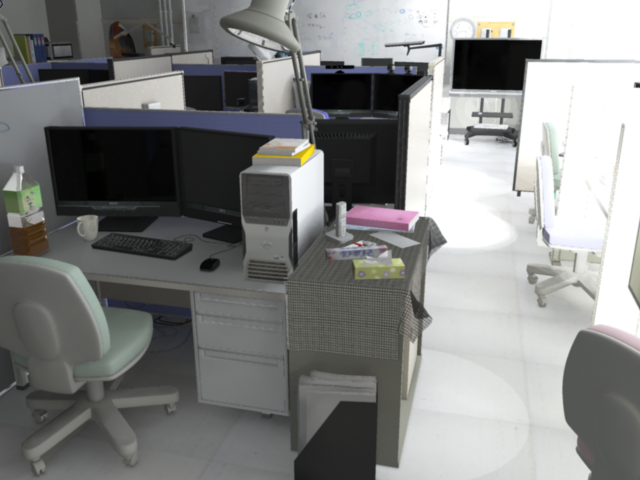
\includegraphics[width=0.25\columnwidth]{./experiments/tsukuba_frame807_rgb.png}
			\end{tabular}
		}\thickspace
		\subfloat[Mapa profundidad LIBELAS]{
			\begin{tabular}[b]{c}
				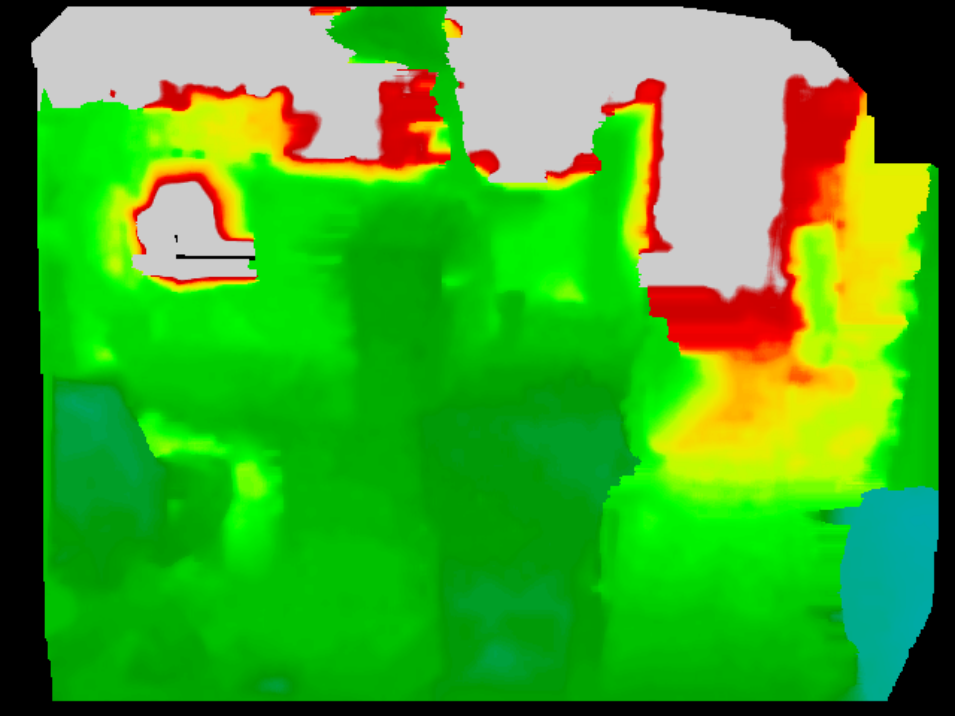
\includegraphics[width=0.25\columnwidth]{./experiments/tsukuba_frame807_libelas_depth_high6.png}
			\end{tabular}
		}\thickspace
		\subfloat[Mapa profundidad S-PTAM Denso]{
			\begin{tabular}[b]{c}
				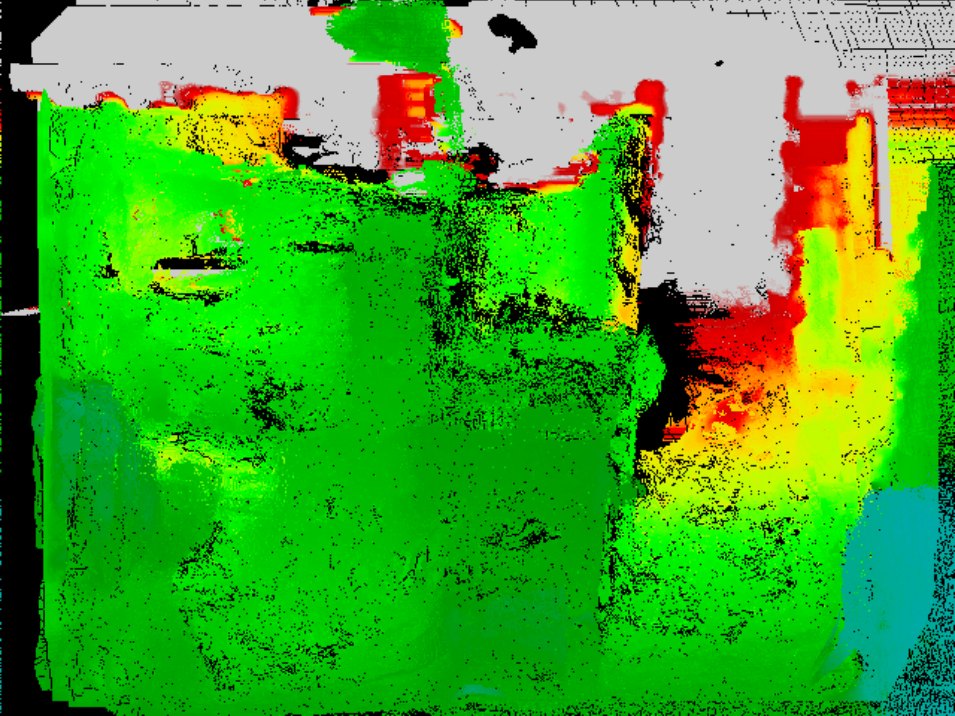
\includegraphics[width=0.25\columnwidth]{./experiments/tsukuba_frame807_dense_high6.png}
			\end{tabular}
		}
	\end{figure}
	\vspace{-2em}
	\begin{figure}
		\captionsetup{justification=centering}
		\subfloat[Ground-Truth]{
			\begin{tabular}[b]{c}
				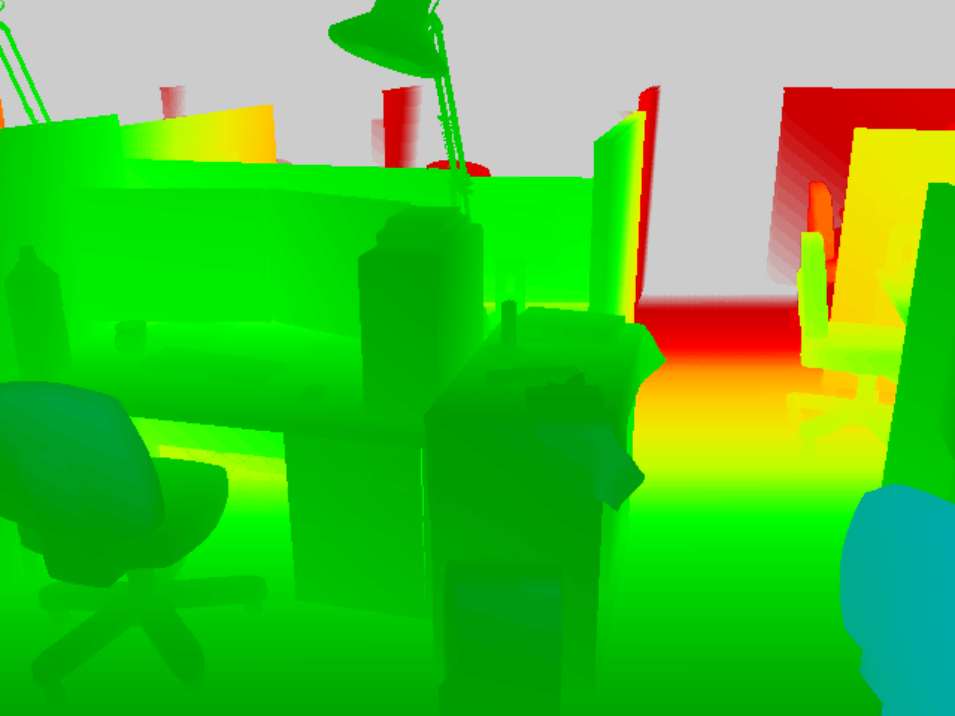
\includegraphics[width=0.25\columnwidth]{experiments/tsukuba_frame807_gt_high6.png}
			\end{tabular}
		}\thickspace
		\subfloat[Error mapa profundidad LIBELAS]{
			\begin{tabular}[b]{c}
				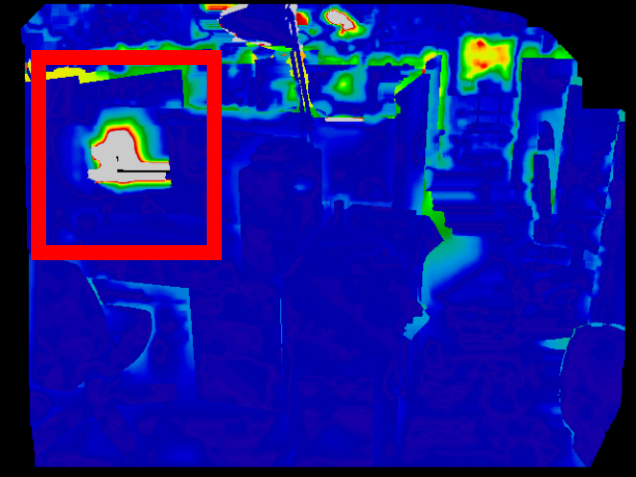
\includegraphics[width=0.25\columnwidth]{./experiments/tsukuba_frame807_libelas_error_high6-m.png}
			\end{tabular}
		}\thickspace
		\subfloat[Error mapa profundidad S-PTAM Denso]{
			\begin{tabular}[b]{c}
				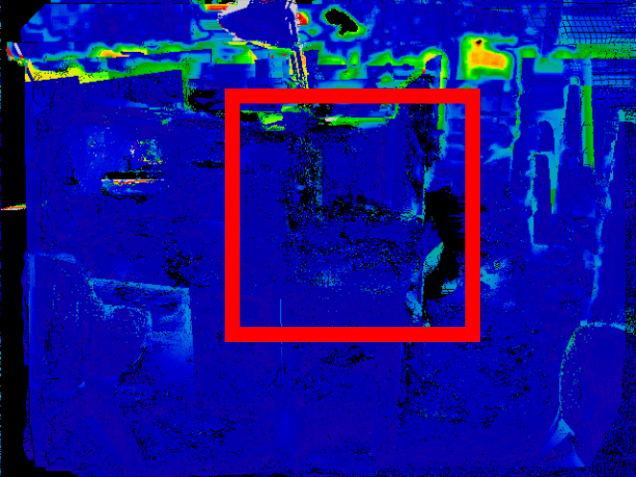
\includegraphics[width=0.25\columnwidth]{./experiments/tsukuba_frame807_error_high6-m.png}
			\end{tabular}
		}
	\end{figure}
	\vspace{-2em}
	\begin{figure}
		\subfloat[]{
			\begin{tabular}[b]{c}
				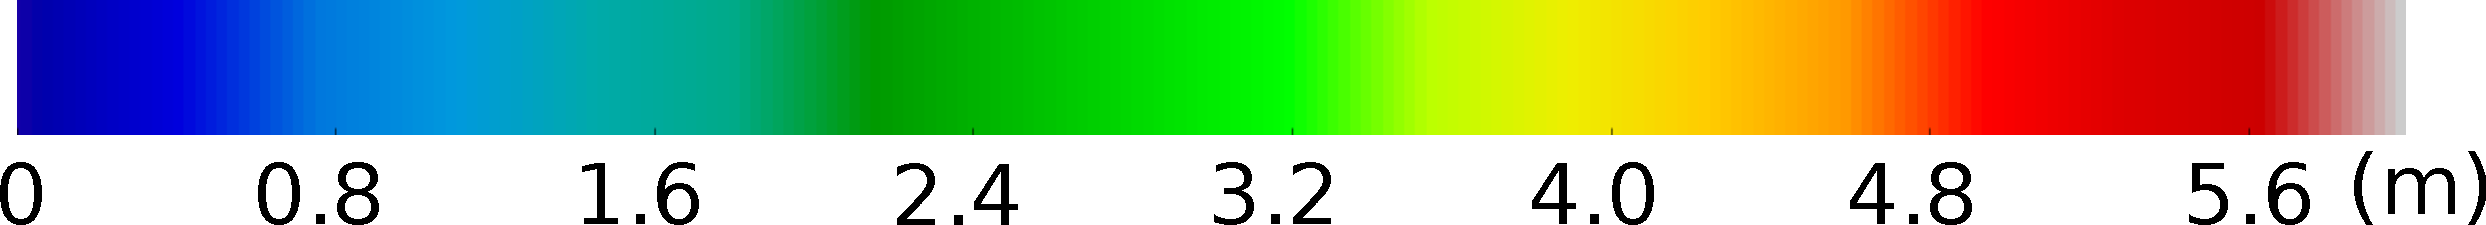
\includegraphics[width=0.60\columnwidth]{./experiments/high6_bar.pdf}
			\end{tabular}
		}
	\end{figure}
\end{frame}


% Frame ---------------------------------------------------------------------
\begin{frame}
	\frametitle{KITTI 06: error de mediana}
	\centering
	Error (profundidad vs. error) en la secuencia 06 del Dataset KITTI.
	\begin{figure}[!htb]
		\captionsetup{justification=centering}
		\subfloat[Error en LIBELAS]{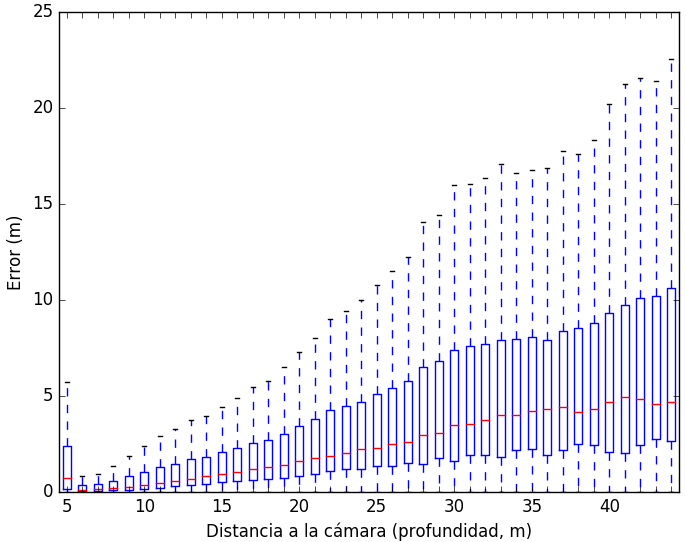
\includegraphics[width=0.48\columnwidth]{./experiments/kitti06_libelas_boxplot.png}%
		}
		\hfil
		\subfloat[Error en S-PTAM Denso]{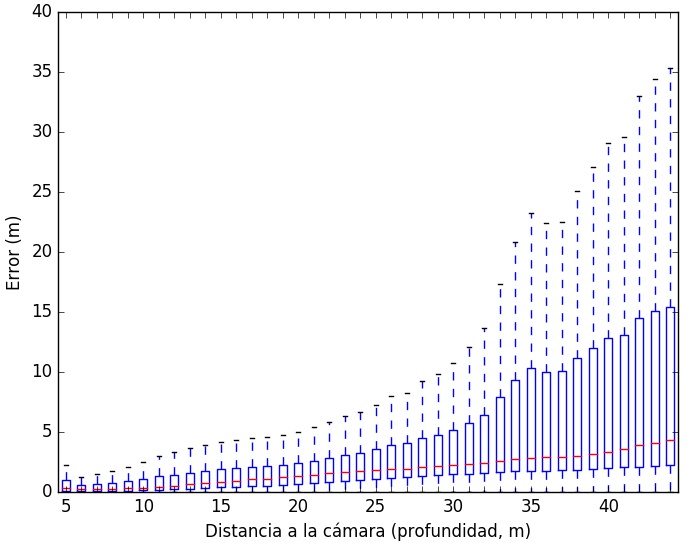
\includegraphics[width=0.48\columnwidth]{./experiments/kitti06_dense_boxplot.png}%
		}
	\end{figure}
\end{frame}


% Frame ---------------------------------------------------------------------
\begin{frame}
	\frametitle{KITTI 06: error de mediana}
	\vspace{-2em}
	\begin{figure}[!htb]
		\captionsetup{justification=centering}
		\subfloat[Comparación de mediana de error entre LIBELAS y S-PTAM Denso (profundidad vs. error) en la secuencia 06 del Dataset KITTI.] {
			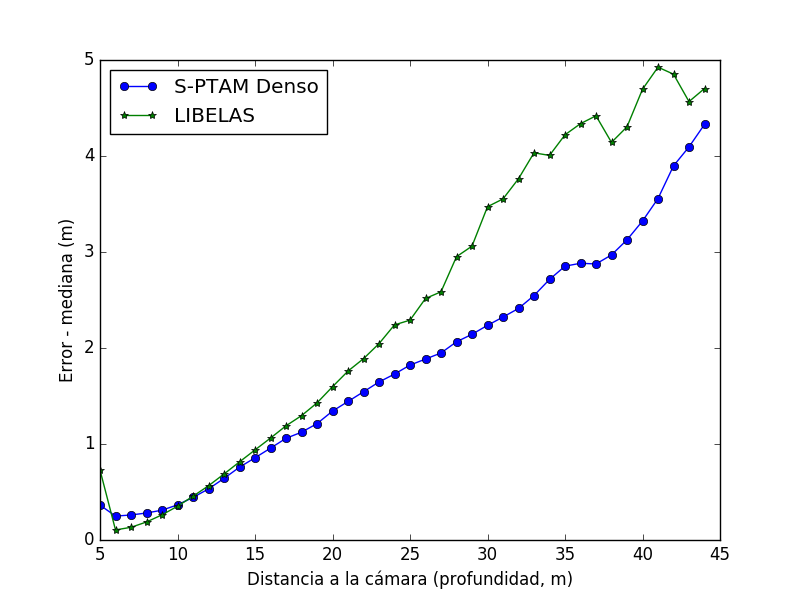
\includegraphics[width=0.8\columnwidth]{./experiments/medians_comparison_kitti.png}%
		}
	\end{figure}
\end{frame}


% Frame ---------------------------------------------------------------------
\begin{frame}
	\frametitle{Tsukuba: error de mediana}
	\centering
	Error (profundidad vs. error) en el Dataset Tsukuba.
	\begin{figure}[!htb]
		\captionsetup{justification=centering}
		\subfloat[Error en LIBELAS]{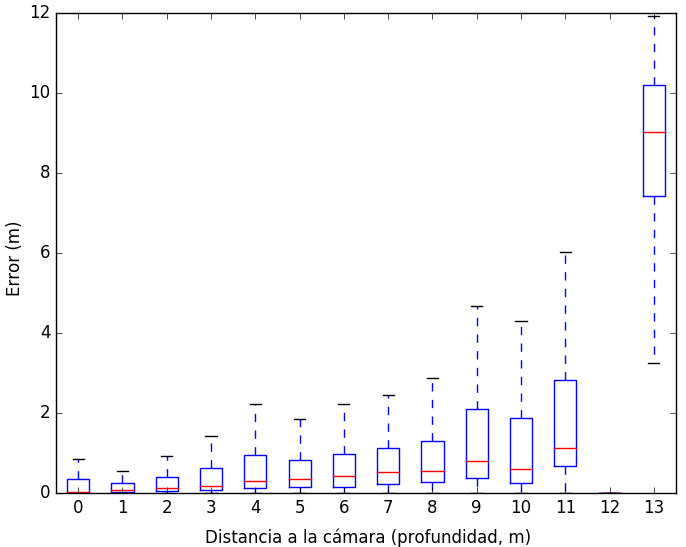
\includegraphics[width=0.48\columnwidth]{./experiments/tsukuba_libelas_boxplot.png}%
		}
		\hfil
		\subfloat[Error en S-PTAM Denso]{\includegraphics[width=0.48\columnwidth]{./experiments/tsukuba_dense_boxplot.png}%
		}
	\end{figure}
\end{frame}


% Frame ---------------------------------------------------------------------
\begin{frame}
	\frametitle{Tsukuba: error de mediana}
	\vspace{-2em}
	\begin{figure}[!htb]
		\captionsetup{justification=centering}
		\subfloat[Comparación de mediana de error entre LIBELAS y S-PTAM Denso (profundidad vs. error) en el Dataset Tsukuba.] {
			\includegraphics[width=0.8\columnwidth]{./experiments/medians_comparison_tsukuba.png}%
		}
	\end{figure}
\end{frame}


% Frame ---------------------------------------------------------------------
\begin{frame}
	\frametitle{KITTI: error de mediana}
	\centering
	Comparación de mediana de error (profundidad vs. error).
	\vspace{-1em}
	\begin{figure}[!htb]
		\captionsetup{justification=centering}
		\subfloat[KITTI 00]{\includegraphics[width=0.35\columnwidth]{./experiments/kitti_medians/00.png}%
		}
		\hfil
		\subfloat[KITTI 01]{\includegraphics[width=0.35\columnwidth]{./experiments/kitti_medians/01.png}%
		}
	\end{figure}
	\vspace{-2em}
	\begin{figure}[!htb]
		\captionsetup{justification=centering}
		\subfloat[KITTI 02]{\includegraphics[width=0.35\columnwidth]{./experiments/kitti_medians/02.png}%
		}
		\hfil
		\subfloat[KITTI 03]{\includegraphics[width=0.35\columnwidth]{./experiments/kitti_medians/03.png}%
		}
	\end{figure}
\end{frame}


% Frame ---------------------------------------------------------------------
\begin{frame}
	\frametitle{KITTI: error de mediana}
	\centering
	Comparación de mediana de error (profundidad vs. error).
	\vspace{-1em}
	\begin{figure}[!htb]
		\captionsetup{justification=centering}
		\subfloat[KITTI 04]{\includegraphics[width=0.35\columnwidth]{./experiments/kitti_medians/04.png}%
		}
		\hfil
		\subfloat[KITTI 05]{\includegraphics[width=0.35\columnwidth]{./experiments/kitti_medians/05.png}%
		}
	\end{figure}
	\vspace{-2em}
	\begin{figure}[!htb]
		\captionsetup{justification=centering}
		\subfloat[KITTI 07]{\includegraphics[width=0.35\columnwidth]{./experiments/kitti_medians/07.png}%
		}
		\hfil
		\subfloat[KITTI 08]{\includegraphics[width=0.35\columnwidth]{./experiments/kitti_medians/08.png}%
		}
	\end{figure}
\end{frame}


% Frame ---------------------------------------------------------------------
\begin{frame}
	\frametitle{KITTI: error de mediana}
	\centering
	Comparación de mediana de error (profundidad vs. error).
	\vspace{-1em}
	\begin{figure}[!htb]
		\captionsetup{justification=centering}
		\subfloat[KITTI 09]{\includegraphics[width=0.35\columnwidth]{./experiments/kitti_medians/09.png}%
		}
		\hfil
		\subfloat[KITTI 10]{\includegraphics[width=0.35\columnwidth]{./experiments/kitti_medians/10.png}%
		}
	\end{figure}
\end{frame}


% Frame ---------------------------------------------------------------------
\begin{frame}
	\frametitle{Cantidad de puntos}
	\begin{figure}[!htb]
		\centering
		\subfloat[KITTI]{\includegraphics[width=0.5\columnwidth]{./experiments/points_kitti06}%
			}
		\hfil
		\subfloat[Tsukuba]{\includegraphics[width=0.5\columnwidth]{./experiments/points_tsukuba}%
			}
	\end{figure}
\end{frame}


% Frame ---------------------------------------------------------------------
\begin{frame}
	\frametitle{Análisis de tiempos}
	\vspace{-0.7em}
	\begin{center}
	\begin{figure}[tbh]
	\begin{centering}
	\begin{tabular}{cccc}
		\toprule 
		Secuencia & Disparidad & Expansión y fusión & Refinamiento\tabularnewline
		\midrule
		\midrule 
		Tsukuba & 118.20 & 132.72 & 4.80\tabularnewline
		\midrule 
		KITTI 00 & 156.92 & 115.40 & 6.53\tabularnewline
		\midrule 
		KITTI 01 & 156.10 & 69.12 & 5.21\tabularnewline
		\midrule 
		KITTI 02 & 160.63 & 108.13 & 6.58\tabularnewline
		\midrule 
		KITTI 03 & 153.66 & 83.01 & 4.83\tabularnewline
		\midrule 
		KITTI 04 & 149.15 & 72.99 & 5.00\tabularnewline
		\midrule 
		KITTI 05 & 165.31 & 108.97 & 5.97\tabularnewline
		\midrule 
		KITTI 06 & 154.89 & 83.21 & 4.84\tabularnewline
		\midrule 
		KITTI 07 & 155.74 & 113.15 & 6.10\tabularnewline
		\midrule 
		KITTI 08 & 152.10 & 101.01 & 5.22\tabularnewline
		\midrule 
		KITTI 09 & 159.84 & 101.20 & 5.76\tabularnewline
		\midrule 
		KITTI 10 & 158.81 & 117.42 & 6.35\tabularnewline
		\bottomrule
	\end{tabular}
	\par\end{centering}
	\centering
	\caption{Tiempo de computación promedio (en ms) para cada fase.}
	\end{figure}
	\par\end{center}
\end{frame}


% Frame ---------------------------------------------------------------------
\begin{frame}
	\frametitle{S-PTAM Denso!}
	\centering
	\inlineMovie[loop&autostart&start=5]{./videos/sptam_dense_online.mp4}{./images/kitti_3d_2}{width=\columnwidth}
\end{frame}


% Frame ---------------------------------------------------------------------
\begin{frame}
	\frametitle{S-PTAM Denso!}
	\centering
	\inlineMovie[loop&autostart&start=5]{./videos/sptam_dense_offline.mp4}{./images/kitti_3d_2}{width=\columnwidth}
\end{frame}


\section{Conclusiones y trabajos futuros}


% Frame ---------------------------------------------------------------------
\begin{frame}
	\frametitle{Conclusiones}
	\begin{itemize}
		\item Sistema de SLAM capaz de generar un \textbf{mapa local denso} en \textbf{tiempo real}.
	    \item Explota paralelismo.
        \item La precisión es útil para tareas de \textbf{navegación}.
        \item Funciona incluso en trajectorias de grandes dimensiones.
        \item Evaluado en datasets públicos: KITTI (outdoors) y Tsukuba (indoors).
	    \item Código open-source en ROS (GPLv3) \url{https://github.com/CIFASIS/dense-sptam}
	    \item Nodo ROS reutilizable, desacoplado del sistema de SLAM disperso.
	\end{itemize}
\end{frame}


% Frame ---------------------------------------------------------------------
\begin{frame}
	\frametitle{Trabajo Futuro}
	\begin{itemize}
		\item Incluir información de apariencia en la heurística.
		\item Ampliar criterio de correspondencias a considerar un entorno alrededor del píxel proyectado.
		\item Simplificar las nubes de puntos mediante la detección de regiones planares.
		\item Características visuales de alto nivel: información semántica y técnicas de machine-learning.
		\item Analizar resultados con otras librerías de disparidad y diferentes métodos de SLAM.
		\item Experimentar sobre otros datasets.
		\item Implementar con soporte para GPU.
	\end{itemize}
\end{frame}


\section*{}


\setbeamercovered{invisible}


% Frame ---------------------------------------------------------------------
\begin{frame}
    \frametitle{Publicaciones}

	\begin{itemize}
		\item A. D'Alessandro, T. Pire, R. Baravalle: \textbf{Hacia una densificación de sistemas SLAM dispersos basados en visión estéreo}. En IX Jornadas Argentinas de Robótica (JAR) 2017. 15, 16 y 17 de Noviembre de 2017. Facultad Regional Córdoba, Córdoba, Universidad Tecnológica Nacional. Noviembre 2017.
		\vspace{1em}
		\item T. Pire, R. Baravalle, A. D'Alessandro, J. Civera: \textbf{Real-time and Locally Dense Stereo SLAM}. En Robotics and Autonomous Systems (RAS). (En revisión).
	\end{itemize}
    
\end{frame}


\begin{frame}
	\centering
	\Large{Muchísimas gracias!}	
	\\
	\pause{Preguntas?}	
	\vspace{2cm}
\end{frame}

\end{document}